\documentclass{beamer}
\usepackage{graphics}
\usepackage{blindtext}
\usepackage{fancybox}
\usepackage{tikz}
\usepackage{caption}
\usepackage{fancybox}
\usepackage{framed}
\usepackage[backend=bibtex, style=numeric, sorting=none]{biblatex}
\addbibresource{/home/gaurish108/Dropbox/MyWiki/research_projects/HorseFly/writeups/horsefly_refs.bib}
\newcommand*{\rom}[1]{\expandafter\@slowromancap\romannumeral #1@}

\usetheme[progressbar=frametitle]{metropolis}
\useoutertheme{metropolis}
\useinnertheme{metropolis}
\usefonttheme{metropolis}
%\usecolortheme{spruce}
\setbeamercolor{background canvas}{bg=white}

\date{}
\title{Package Delivery with Trucks and Drones: The Horsefly Problem} 
\subtitle{}
\author{Joseph S. B. Mitchell, \hspace{2pt} Gaurish Telang}
\institute{ \vspace{-8pt} Stony Brook University, New York \\\vspace{9pt}
{\textit{\tiny(In collaboration with Sujoy Bhore, John Gunnar Carlsson, S\'andor Fekete)}}  \\ \\ Fall Workshop in Computational Geometry, 2018 \\ }
\begin{document}
\metroset{block=fill}


%%%%%%%%%%%%%%%%%%%%%%%%%%%%%%%%%%%%%%%%%%%%%%%%%%%%%%%%%%%%%%%%%%%%%%%%%%%%%%%%%%%%%%%%%%%%%%%%%%
\begin{frame}
  \titlepage
vspace{2mm}

\end{frame}
%%%%%%%%%%%%%%%%%%%%%%%%%%%%%%%%%%%%%%%%%%%%%%%%%%%%%%%%%%%%%%%%%%%%%%%%%%%%%%%%%%%%%%%%%%%%%%%%%%
% For the most part follow the presentation given 
% in the FWCG submission. Throw in a few interesting
% examples for good measure, along with conjectures,
% future-work yada, yada. When no obstacles involved
% point out that a realistic setting would involve
% obstacles, or road=network...Add to last section
% maybe? 
\begin{frame}[t]{Using Trucks and Drones in Tandem} \vspace{-25pt}
  \begin{columns}
    \begin{column}{0.45\textwidth}
      \begin{figure}
        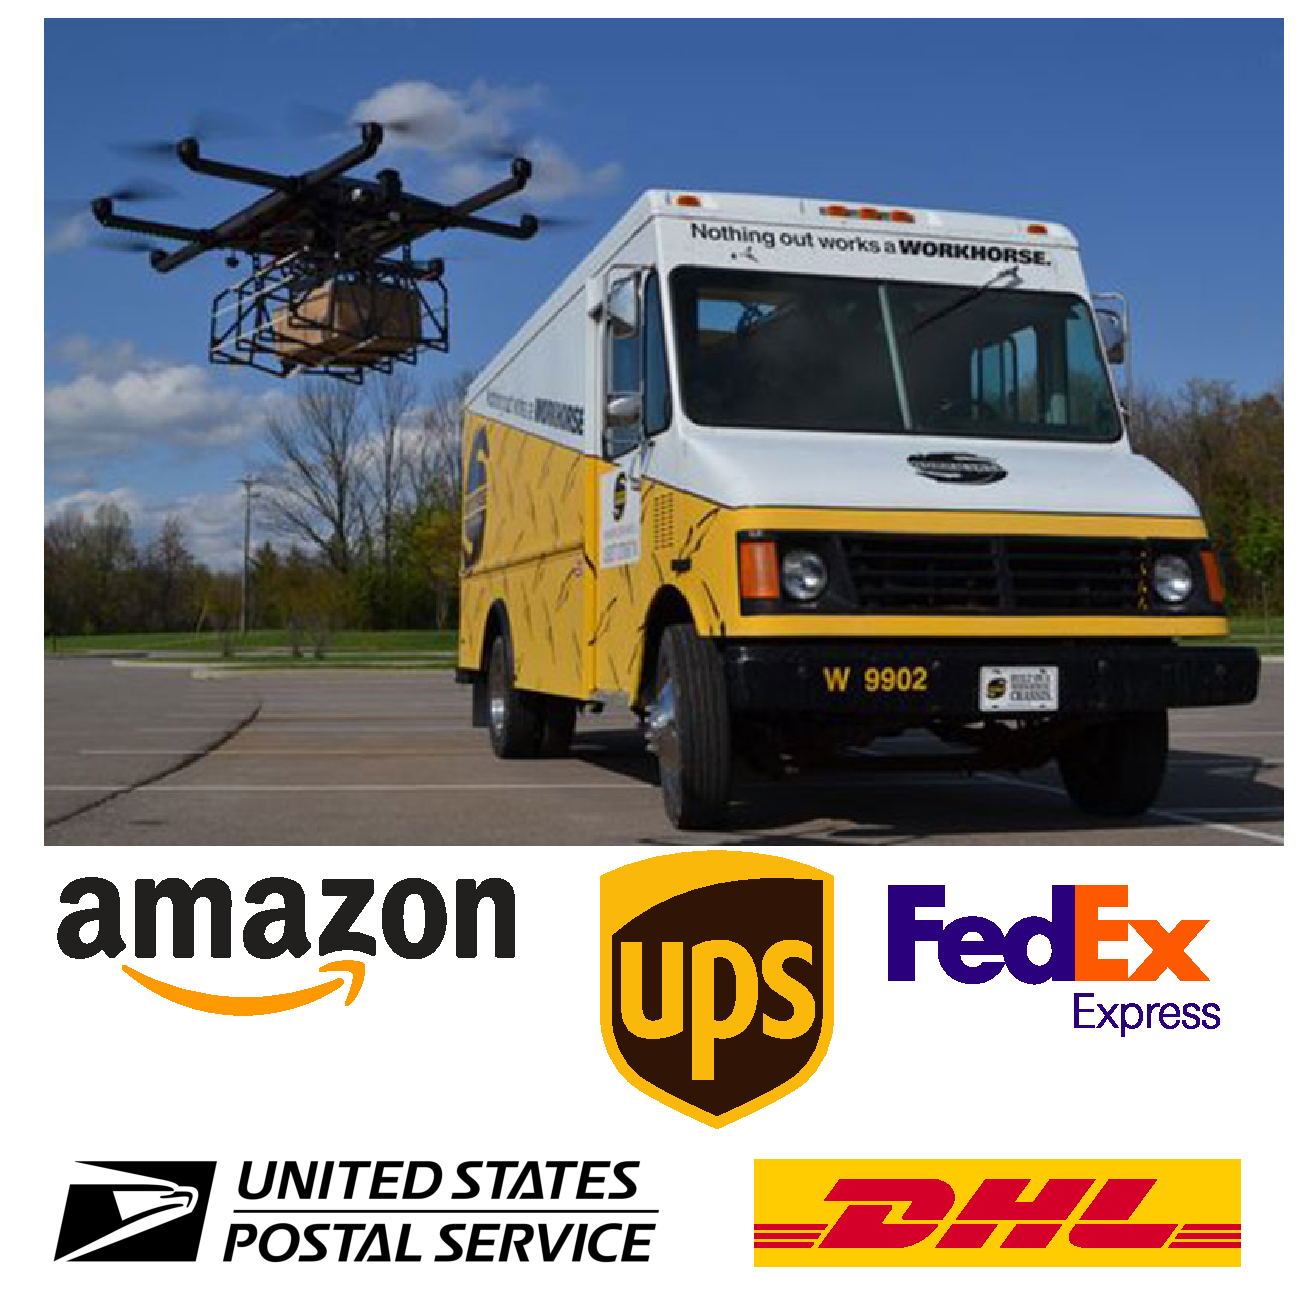
\includegraphics[width=6.0cm]{slide_imgs/introslide_image.eps}
      \end{figure}
    \end{column}

    \begin{column}{0.55\textwidth}
      \vspace{25pt}
      \begin{quote}
      ``UPS has estimated
  that cutting off just one mile for the routes of each of the
  company's 66,000 delivery drivers would amount to   {\color{red}   \$50 million } in
  savings. For this reason, UPS is testing drone deliveries, using the
  top of its vans as a mini-helipad.'' \footnotemark
  \end{quote}
    \end{column}
  \end{columns}
 \vspace{2mm}
  \footnotetext[1]{ From \url{https://www.businessinsider.com/amazon-and-ups-are-betting-big-on-drone-delivery-2018-3}}
\end{frame}

%%%%%%%%%%%%%%%%%%%%%%%%%%%%%%%%%%%%%%%%%%%%%%%%%%%%%%%%%%%%%%%%%%%%%%%%%%%%%%%%%%%%%%%%%%%%%%%%%%

\begin{frame}{Statement of Horsefly-PATH}
  \begin{columns}
    \begin{column}{0.5\textwidth}
    % A sample image dscribing horsefly path
    \vspace{-19pt}
    \begin{figure}
      \only<1>{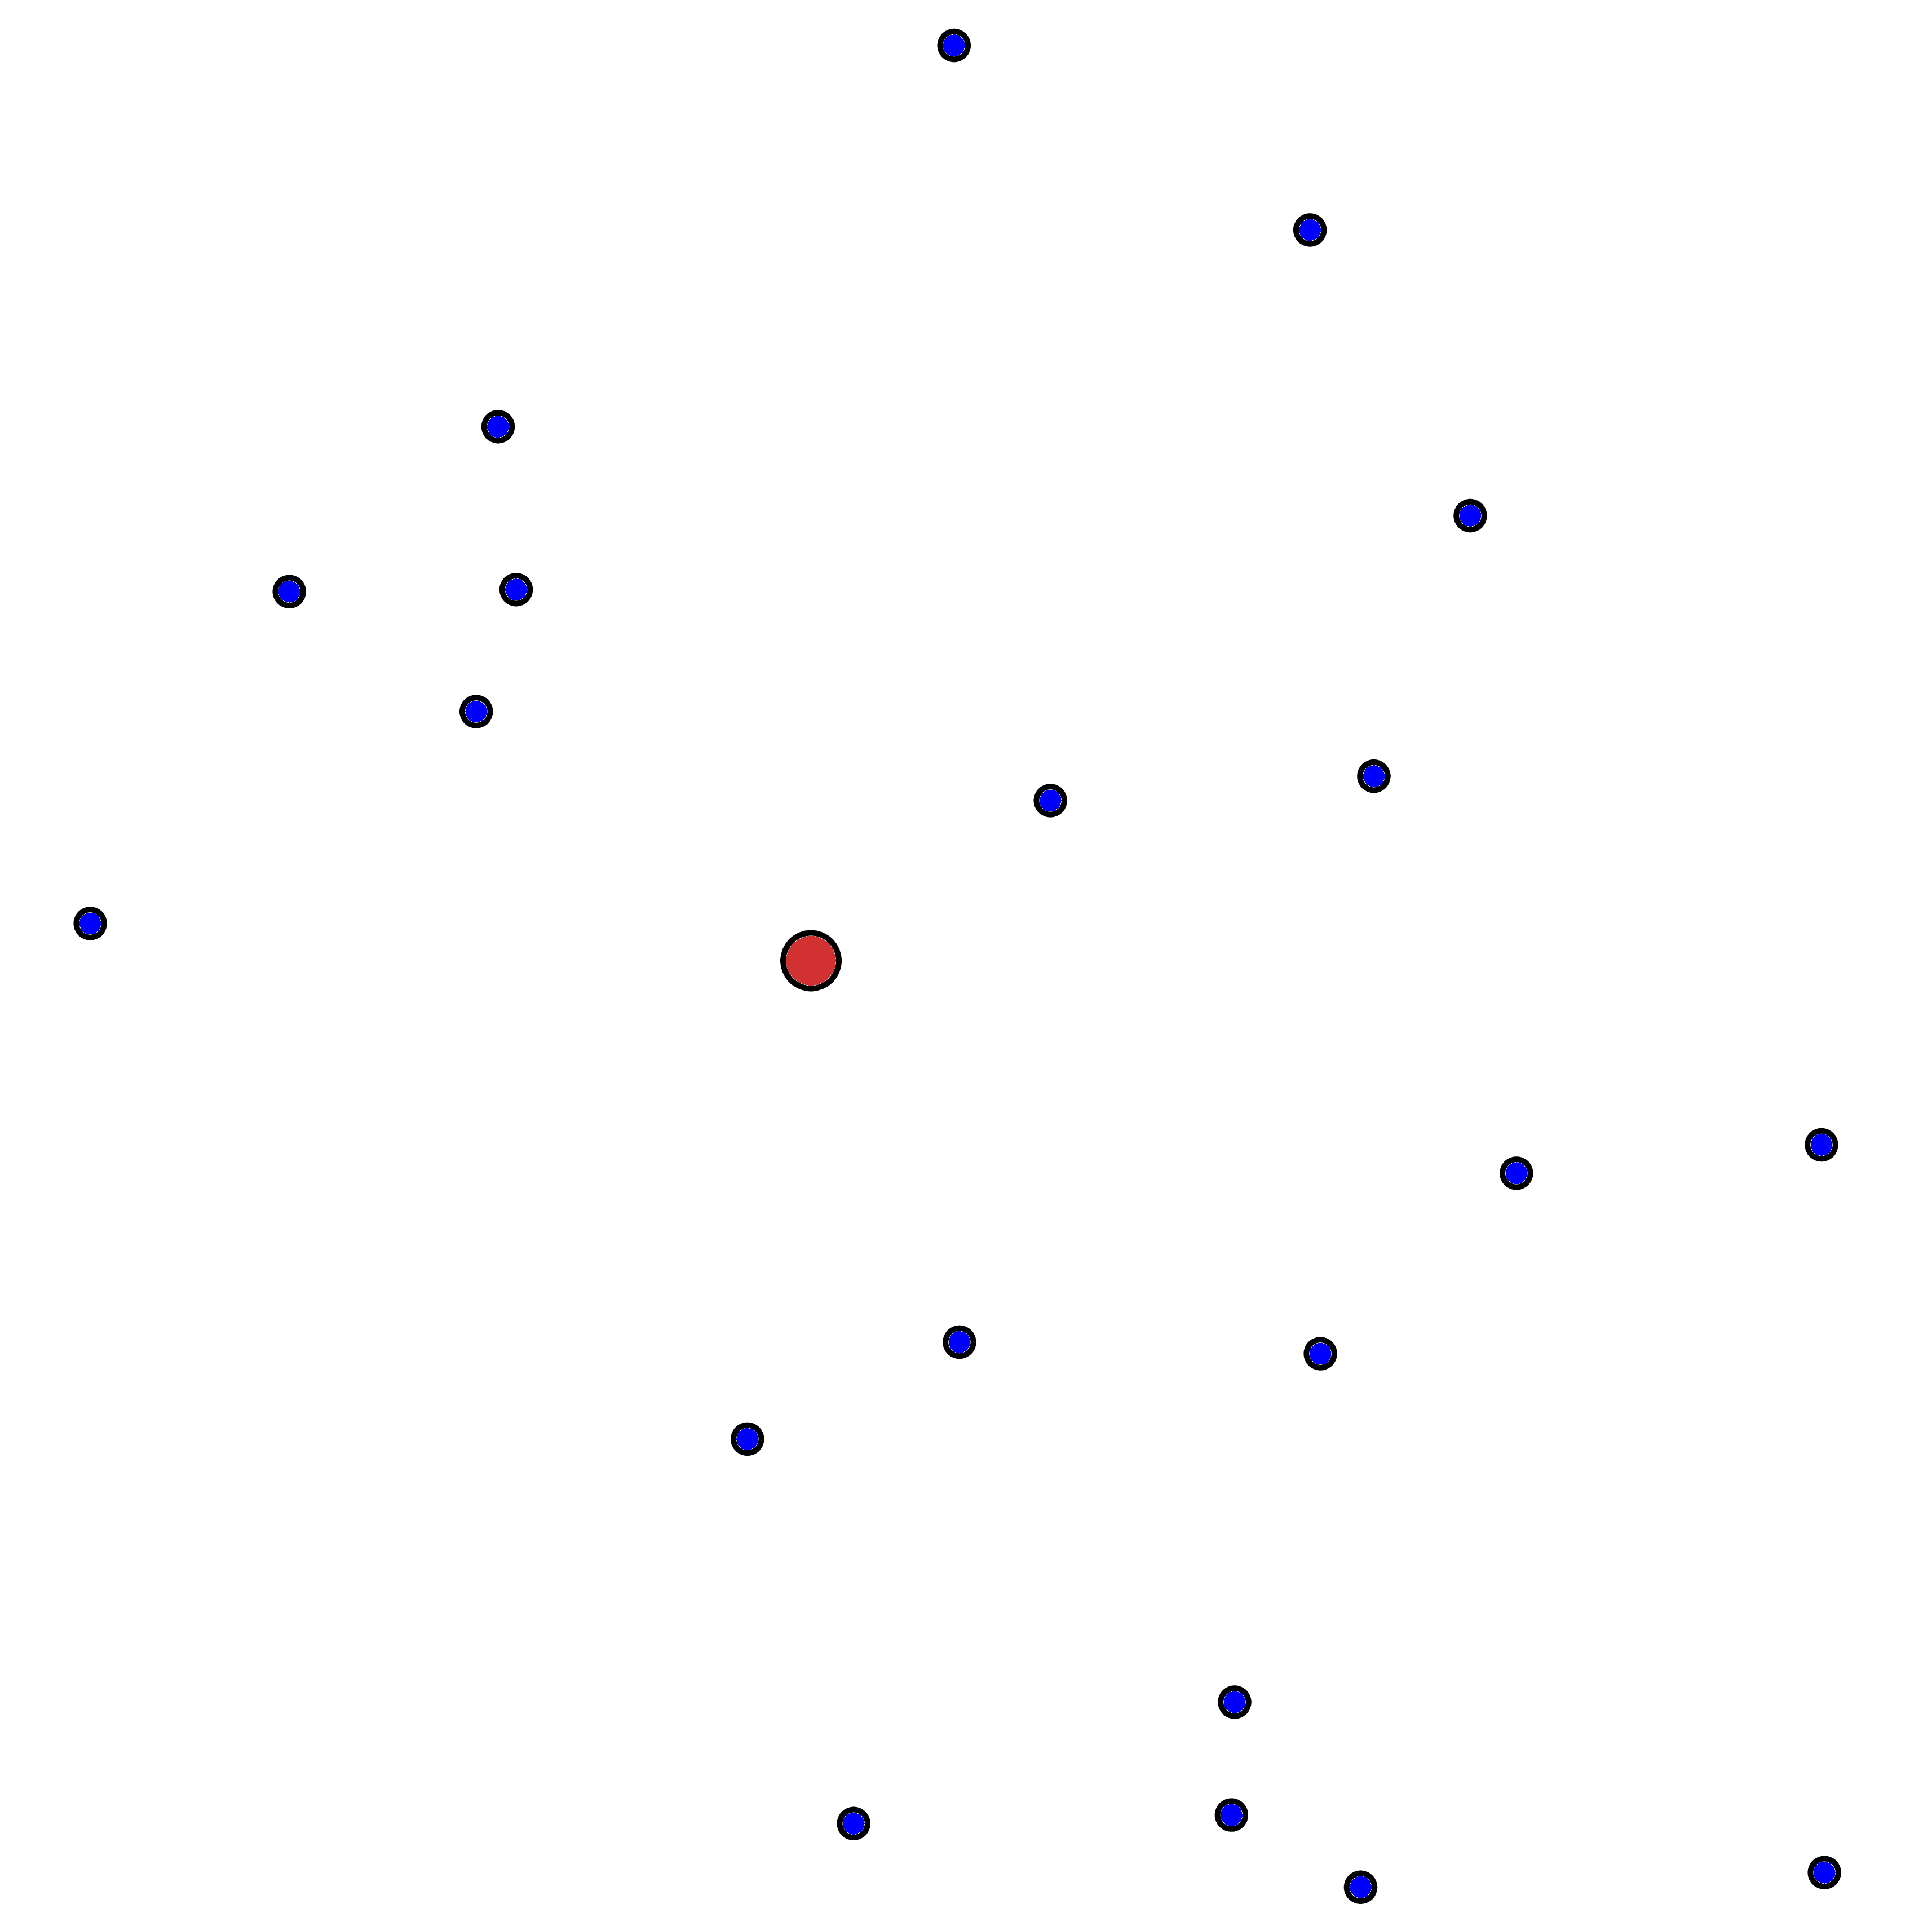
\includegraphics[width=6cm]{slide_imgs/horsefly_demo_input.jpg}}
      \only<2>{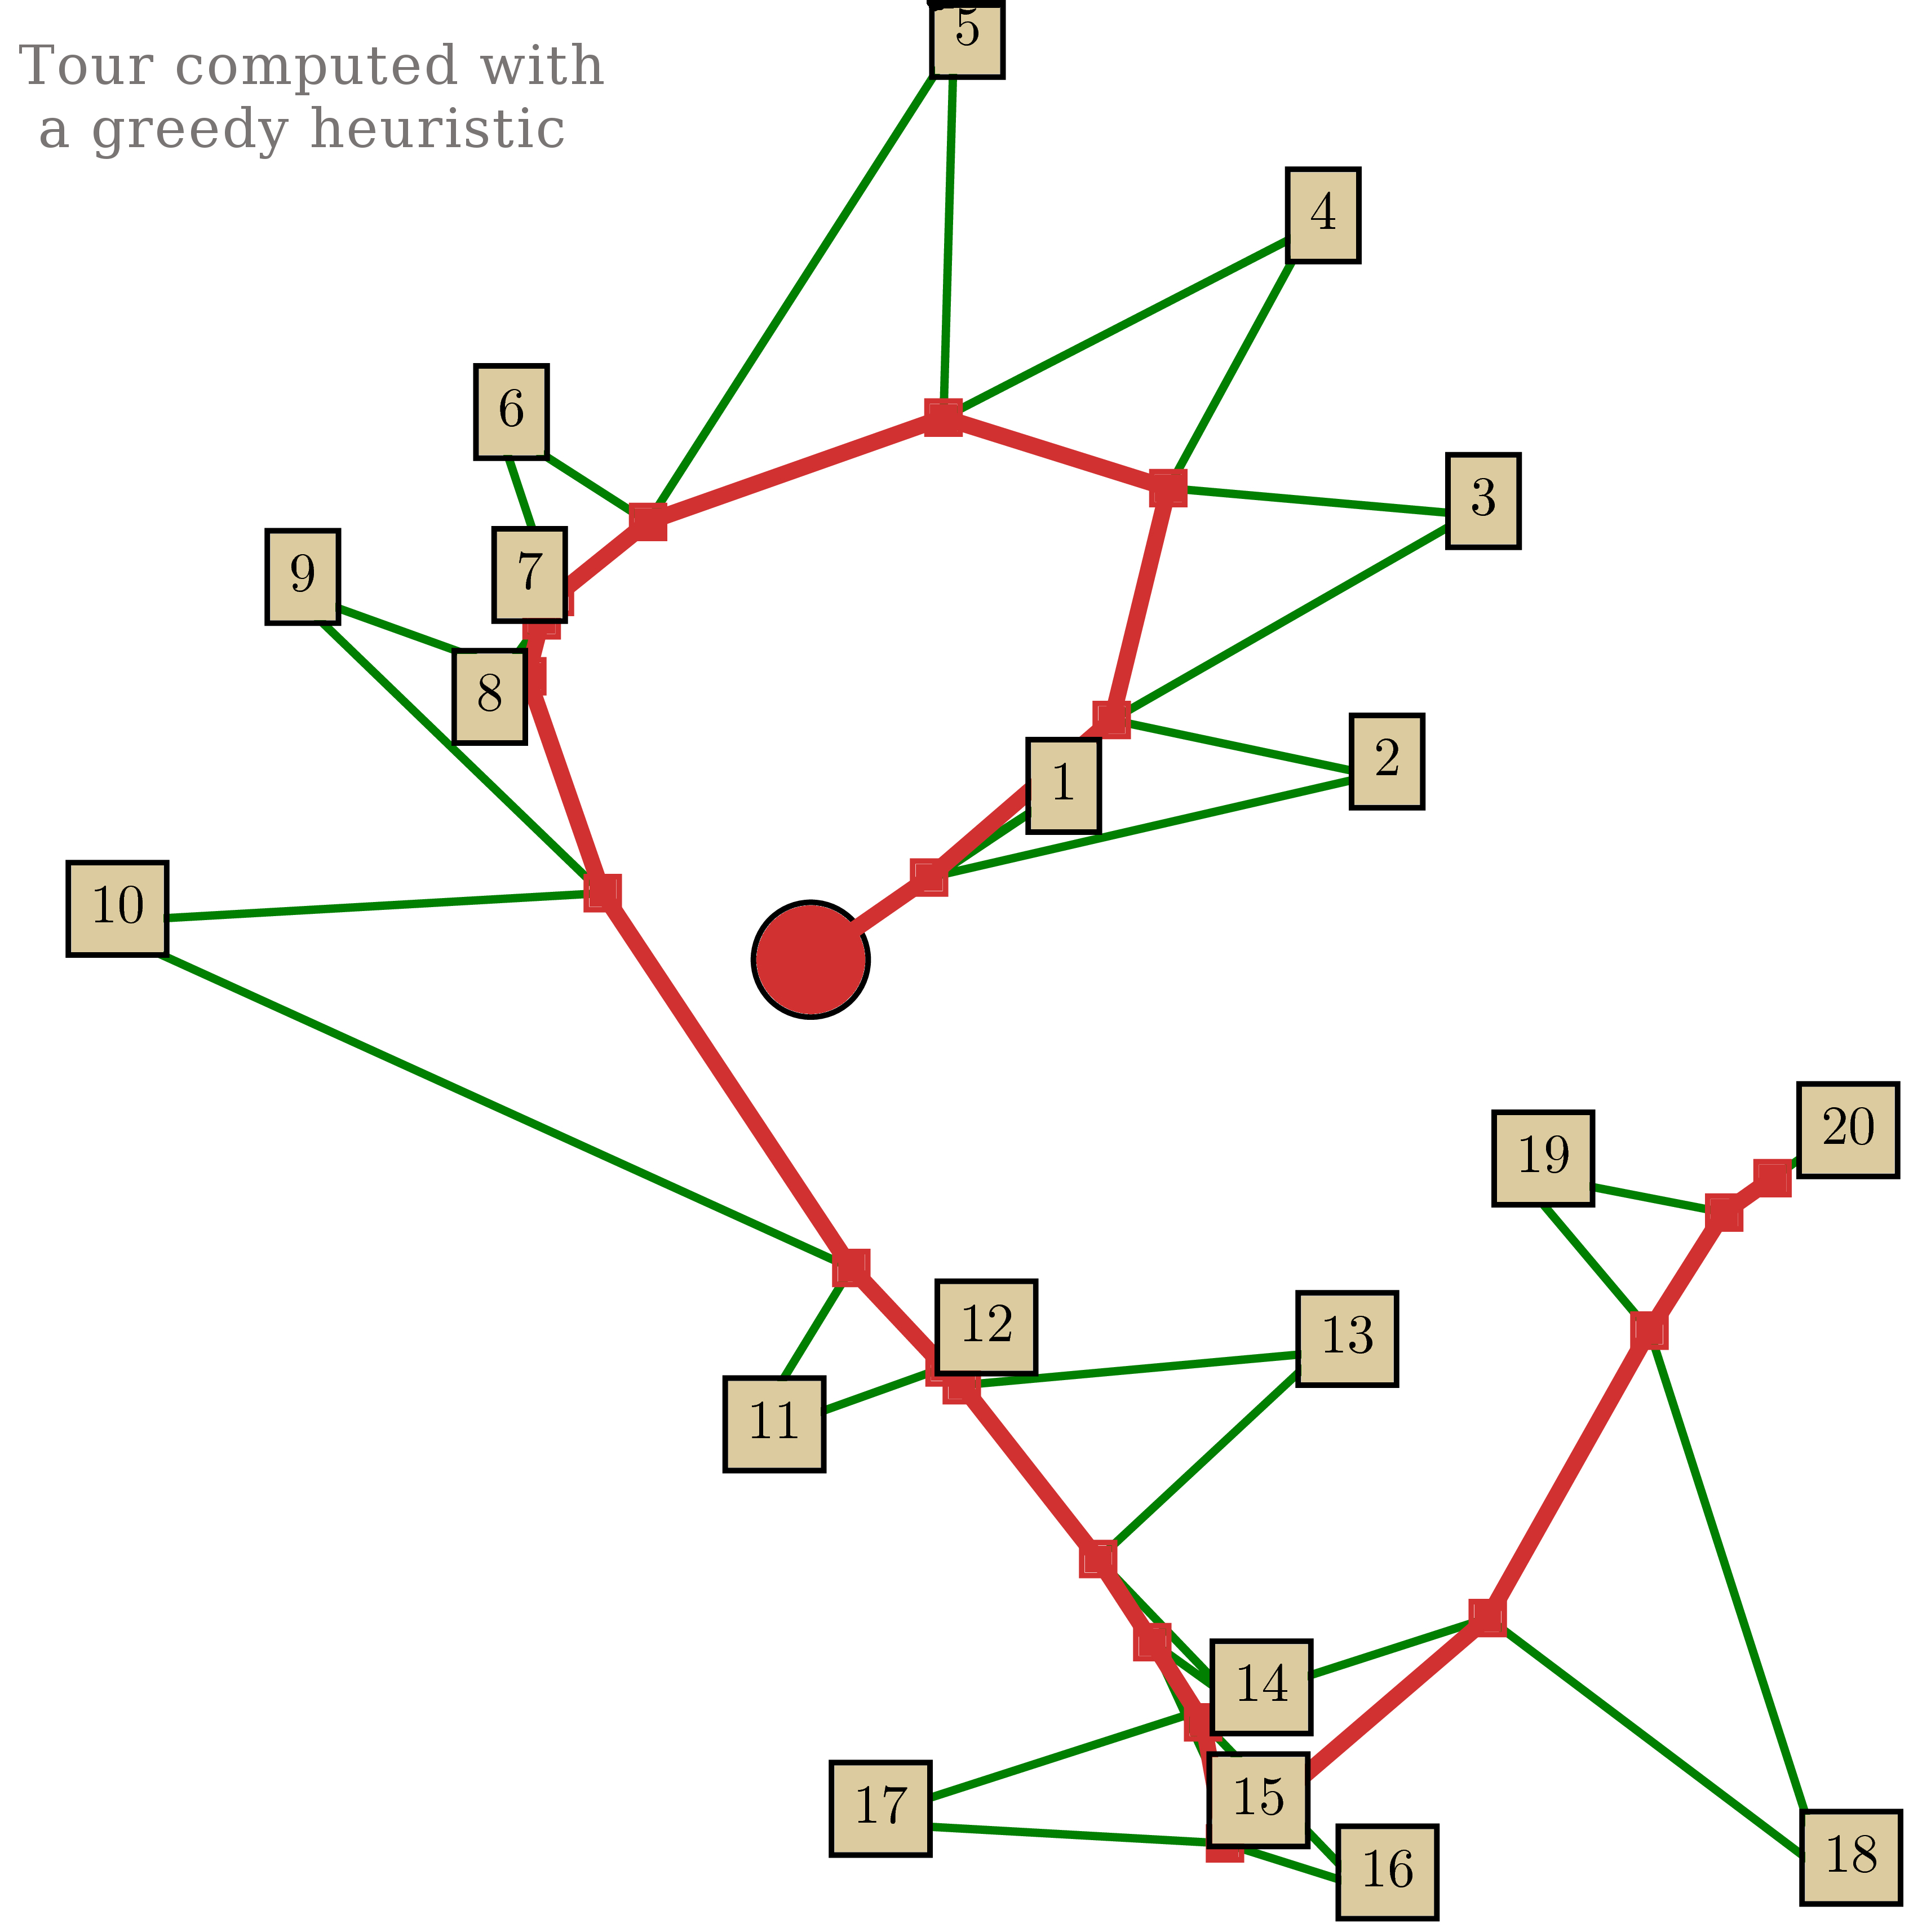
\includegraphics[width=6cm]{slide_imgs/horsefly_demo_output.jpg}}
    \end{figure}
    
    {\small
      \vspace{-15pt}
      \definecolor{dronegreen}{rgb}{0.0, 0.5, 0.0}
      \hspace{40pt} Speed Ratio \varphi = 3.0 \\
      \hspace{40pt} Truck Path : \tikz[baseline=-0.5ex]{ \draw[red, thick] [-] (0,0) -- (5ex,0); }  \\
      \hspace{40pt} Drone Path : \tikz[baseline=-0.5ex]{ \draw[dronegreen, thick] [-] (0,0) -- (5ex,0); }  \\
     } 
    \end{column}

    \begin{column}{0.5\textwidth}
      \begin{center}
        
      \begin{figure}
        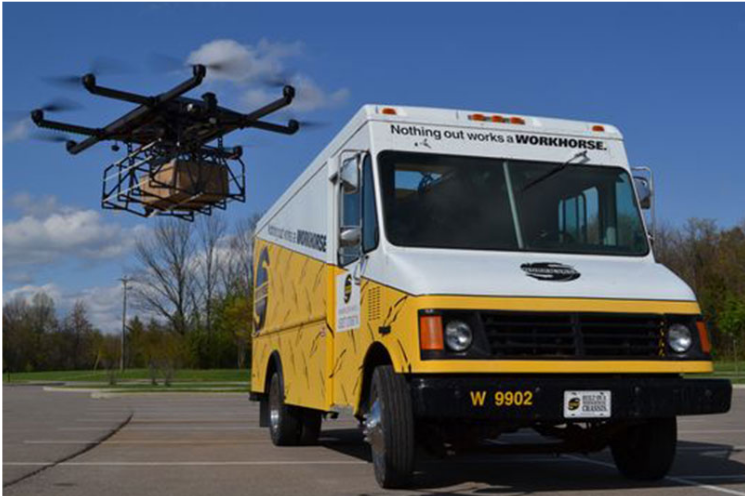
\includegraphics[width=2.0cm]{slide_imgs/small_truck_and_drone.png}
      \end{figure}
        Compute a route for the truck and for the drone in order to complete the delivery of
        all $n$ packages (and have the drone return back to the empty truck)
        was soon as possible i.e., we seek to {\color{red} minimize  makespan} of the delivery process.

        \vspace{-12pt}
        \begin{framed}
        Both the {\color{red} order} of visiting the sites  
        \underline{and} {\color{red} Steiner points} need to be computed!
        \end{framed}
        
       \end{center}
    \end{column}
    
  \end{columns}
\end{frame}


%%%%%%%%%%%%%%%%%%%%%%%%%%%%%%%%%%%%%%%%%%%%%%%%%%%%%%%%%%%%%%%%%%%%%%%%%%%%%%%%%%%%%%%%%%%%%%%%%%%%%%%

\begin{frame}{Preliminary Notes}
    \begin{columns}
    \begin{column}{0.5\textwidth}
      % A sample image dscribing horsefly path
      \vspace{-19pt}
    \begin{figure}
      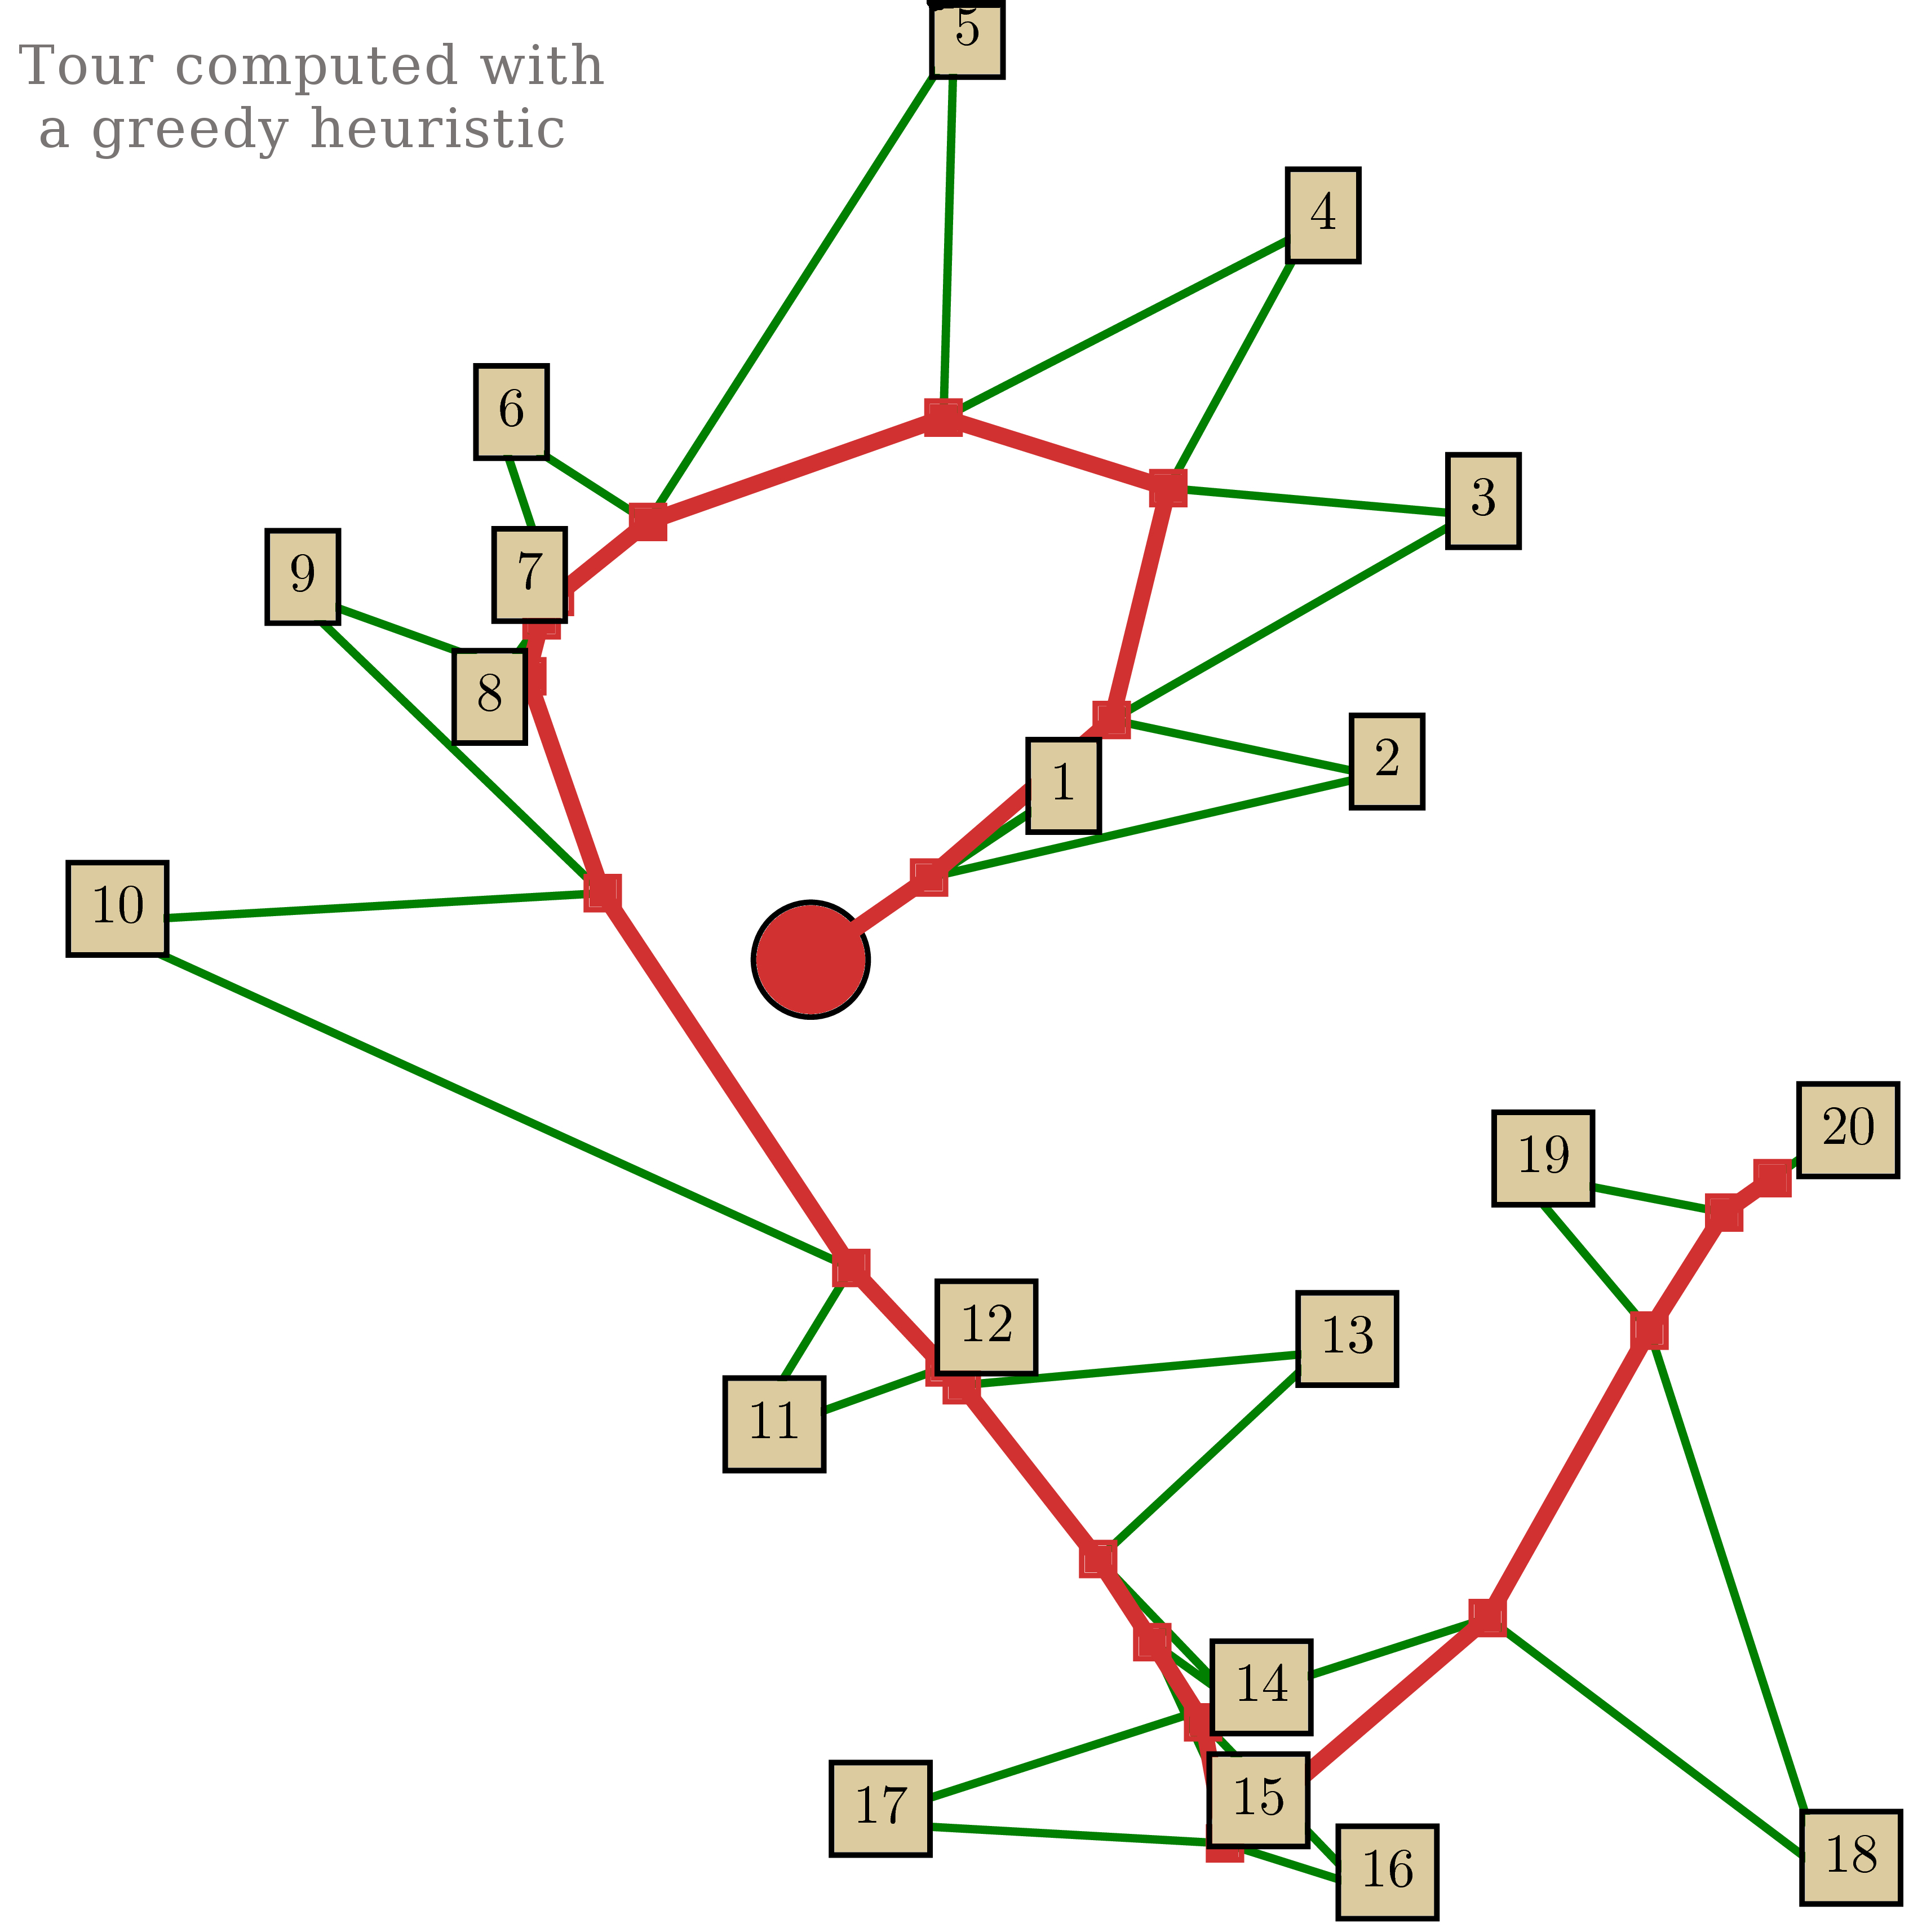
\includegraphics[width=6cm]{slide_imgs/horsefly_demo_output.jpg}
    \end{figure}

    
    {\small
      \vspace{-15pt}
      \definecolor{dronegreen}{rgb}{0.0, 0.5, 0.0}
      \hspace{40pt} Speed Ratio \varphi = 3.0 \\
      \hspace{40pt} Truck Path : \tikz[baseline=-0.5ex]{ \draw[red, thick] [-] (0,0) -- (5ex,0); }  \\
      \hspace{40pt} Drone Path : \tikz[baseline=-0.5ex]{ \draw[dronegreen, thick] [-] (0,0) -- (5ex,0); }  \\
     } 
    \end{column}

   \begin{column}{0.5\textwidth}
      \begin{itemize}
       \item[(1)] Horsefly is {\color{red} NP-hard}, by reduction from TSP ($\varphi = 1.0$)
       \item[(2)] Truck or drone {\color{red} never wait} in OPT for Horsefly-PATH. 
       \item[(3)] The truck route and the drone route are {\color{red} polygonal}
       \item[(4)] The truck and the drone move always at their {\color{red} maximum speeds}(1 and $\varphi$, respectively).
      \end{itemize}
    \end{column}
    
  \end{columns}
       
\end{frame}


%%%%%%%%%%%%%%%%%%%%%%%%%%%%%%%%%%%%%%%%%%%%%%%%%%%%%%%%%%%%%%%%%%%%%%%%%%%%%%%%%%%%%%%%%%%%%%%%%%
% Place a TikZ pictures.
\begin{frame}{Preliminary Notes: Optimal Order depends on $\varphi$}
  \begin{center}

    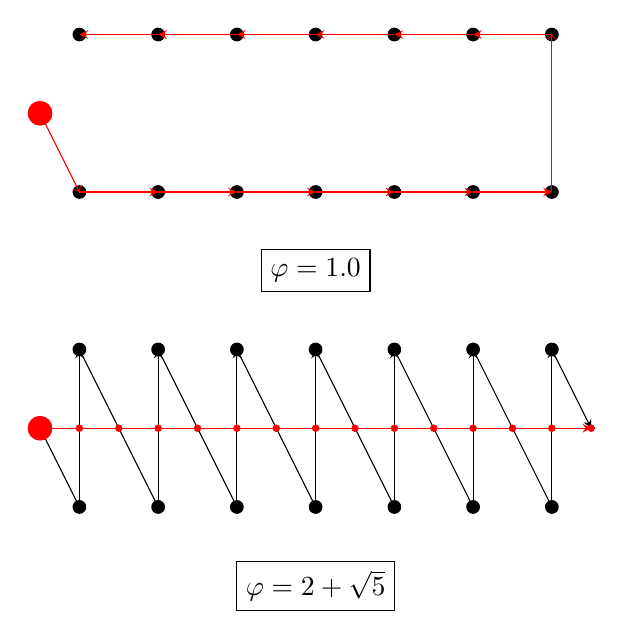
\begin{tikzpicture}
      %%%%%%%%%%%%%%%%%%%%%%%%%%%%%%%%%%%%%%%%%%%%%%
      %%% When speed ration is 1.0, follow TSP path
      %%%%%%%%%%%%%%%%%%%%%%%%%%%%%%%%%%%%%%%%%%%%%
     \foreach \x in {0,...,6} % top row of sites
         \draw[fill] (\x,4) circle (0.08cm);
     \foreach \x in {0,...,6} % bottom row of sites
         \draw[fill] (\x,6) circle (0.08cm);
     % Path of the horse. Draw it as red.
     \foreach \x in {0,...,5}
          \draw [->, red , >=stealth]  (\x,4) -- (\x+1,4); 
          
     \foreach \x in {0,...,5}
          \draw [<-, red , >=stealth]  (\x,6) -- (\x+1,6); 
      % Path of the drone
      \draw [->, red] (-0.5,5) -- (0,4);
      \draw [->, red] (6,4) -- (6,6);

      
     % Assume there are lots of sites to the right
     %\node[draw=none] (ellipsis1) at (7,5) {$\cdots$};

     % Initial position of the horse and fly.
     \draw[fill, red] (-0.5,5) circle (0.15cm); 
      \node[draw,align=center] at (3,3) {$\varphi = 1.0$};
      %%%%%%%%%%%%%%%%%%%%%%%%%%%%%%%%%%%%%%%%%%
      %%% When speed ratio is not 1.0
      %%%%%%%%%%%%%%%%%%%%%%%%%%%%%%%%%%%%%%%%%%
     \foreach \x in {0,...,6} % top row of sites
         \draw[fill] (\x,0) circle (0.08cm);
     \foreach \x in {0,...,6} % bottom row of sites
         \draw[fill] (\x,2) circle (0.08cm);
      % Path of the drone
      \draw [->] (-0.5,1) -- (0,0);
      \foreach \x in {0,...,6}
          \draw [->, >=stealth]  (\x,0) -- (\x,2);    
      \foreach \x in {0,...,5}
          \draw [->]  (\x,2) -- (\x+1,0); 
      \draw [->, >=stealth] (6,2) -- (6.5,1); 
      % Rendezvous points
      \foreach \x in {0,...,6}
      {\draw [fill, red]  (\x,1) circle (0.04cm);
        \draw [fill, red]  (\x+0.5,1) circle (0.04cm);
      }
      % Initial position of the horse and fly.
     \draw[fill, red] (-0.5,1) circle (0.15cm); 
      % Path of the horse
     \draw[->, red, >=stealth] (-0.5,1) -- (6.5,1) ;
     % Assume there are lots of sites to the right
     %\node[draw=none] (ellipsis1) at (7,1) {$\cdots$};

      \node[draw,align=center] at (3,-1) {$\varphi = 2 + \sqrt{5}$};
   \end{tikzpicture}

   
   \end{center}

  
\end{frame}

%%%%%%%%%%%%%%%%%%%%%%%%%%%%%%%%%%%%%%%%%%%%%%%%%%%%%%%%%%%%%%%%%%%%%%%%%%%%%

\begin{frame}[fragile]{Preliminary Notes: Optimal Order depends on $\varphi$}
  \begin{figure}
    \centering
    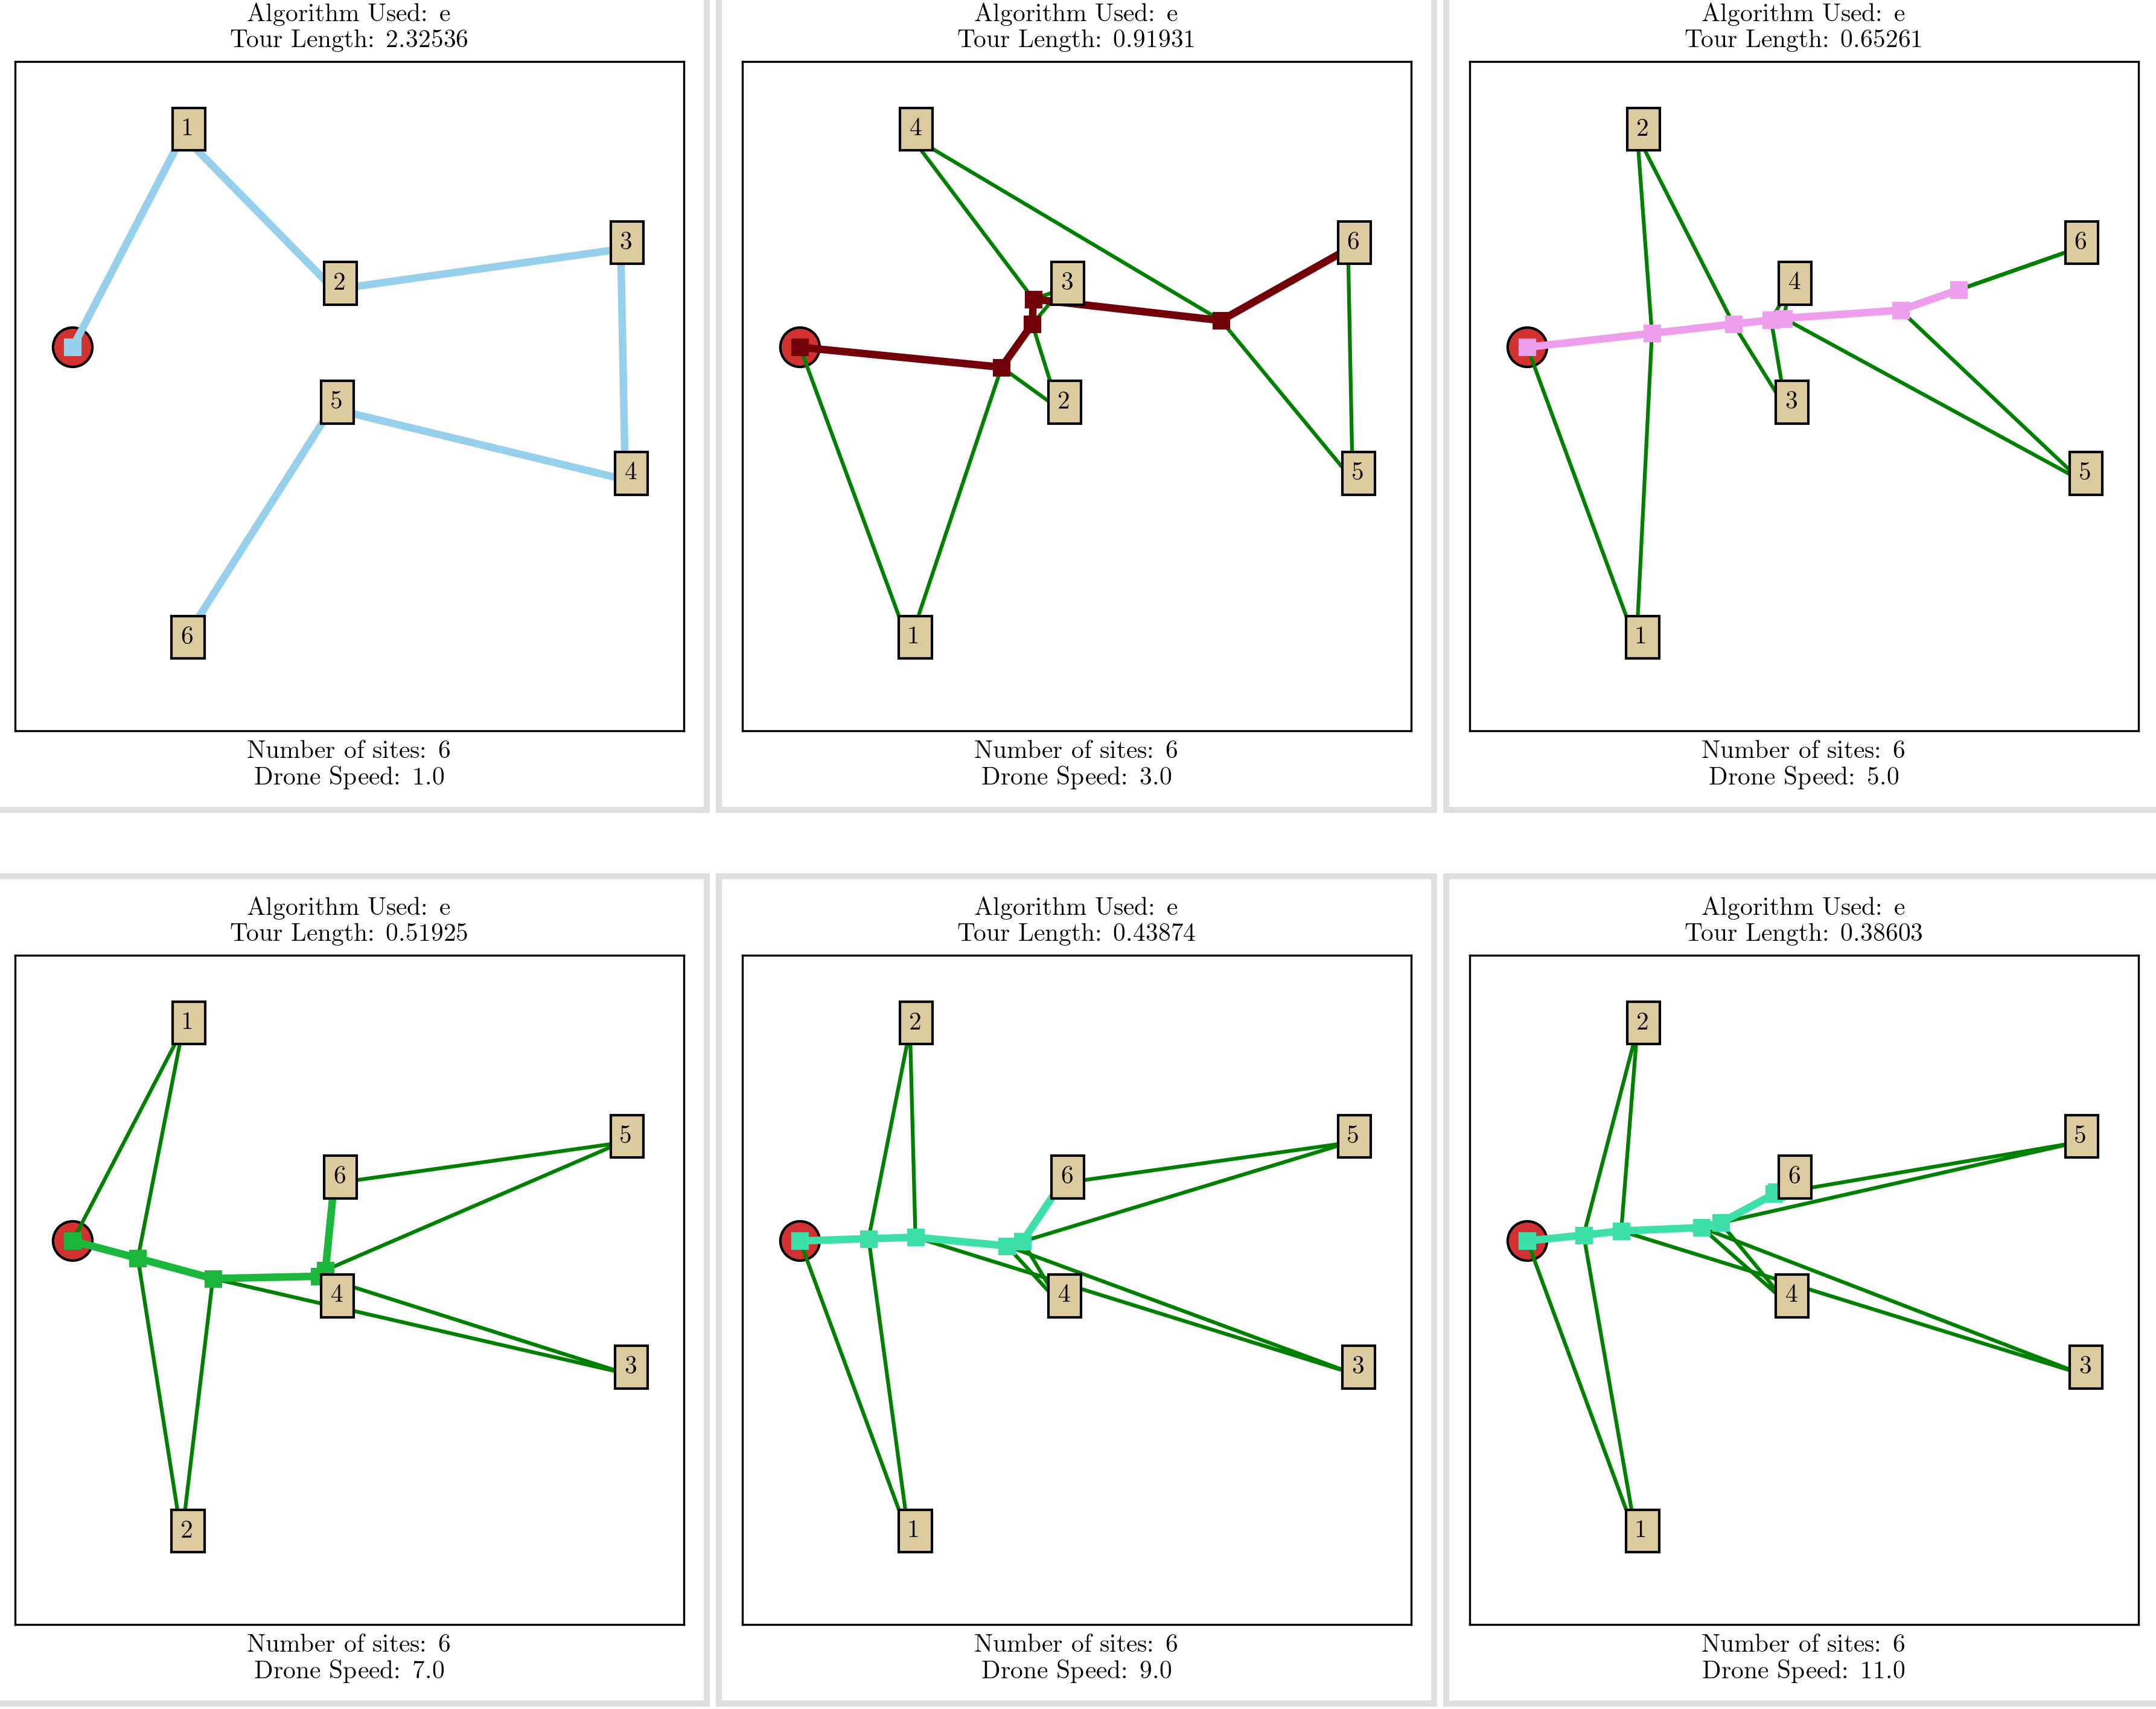
\includegraphics[width=10.5cm]{slide_imgs/exact_different_drone_speeds.png}
  \end{figure}

%\vspace{-15pt} 
%\definecolor{coolgrey}{rgb}{0.55, 0.57, 0.67}
%{\color{coolgrey} {\tiny 
%  \begin{verbatim}
%   Show Movie: gnome-open output-exact.mp4&
%  \end{verbatim} } }
  
\end{frame}

%%%%%%%%%%%%%%%%%%%%%%%%%%%%%%%%%%%%%%%%%%%%%%%%%%%%%%%%%%%%%%%%%%%%%%%%%%%%

\begin{frame}[t]{Preliminary Notes: A Local Optimality Condition}
 \begin{figure}
    \centering
    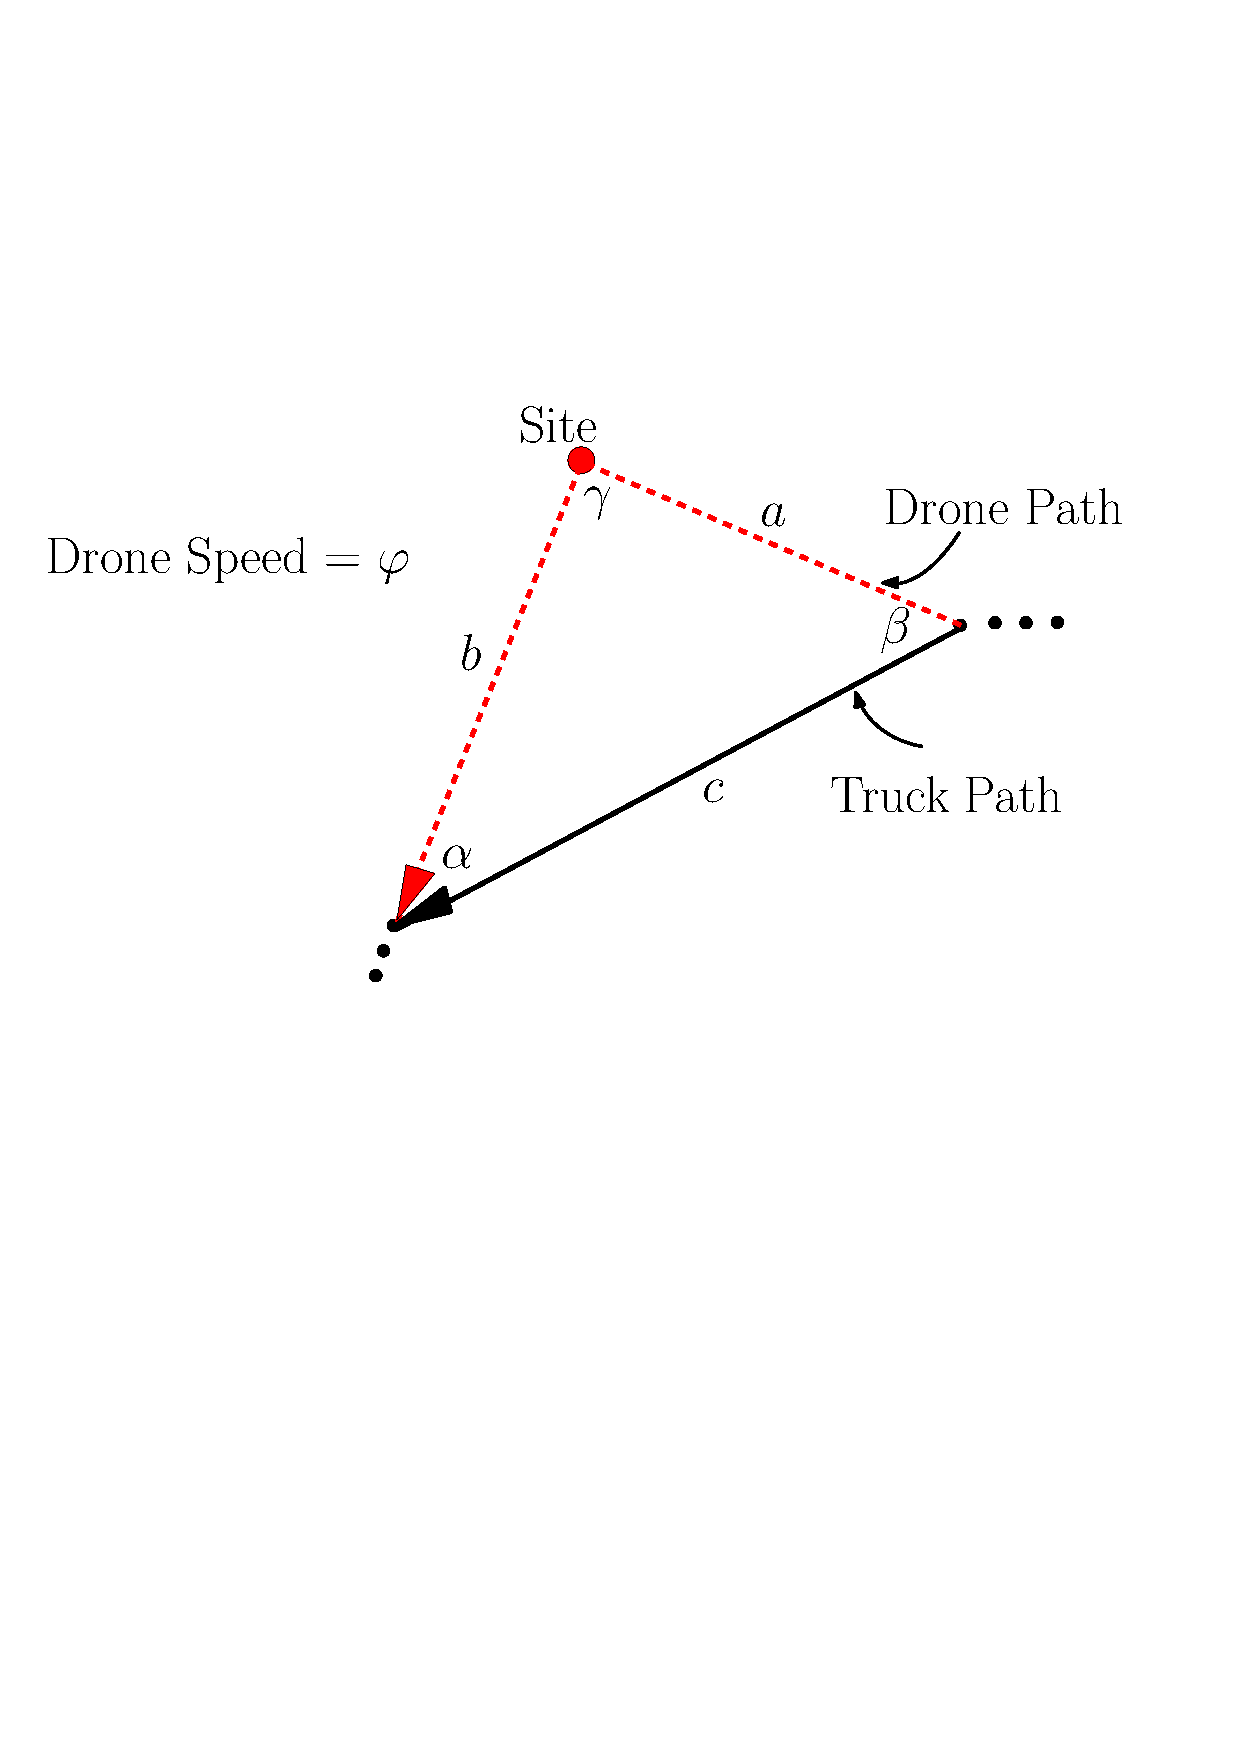
\includegraphics[width=10cm]{slide_imgs/locopt.pdf}
 \end{figure}

 \begin{center}
   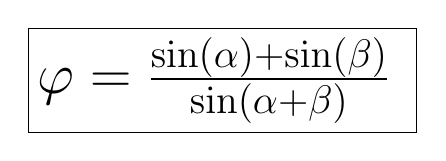
\begin{tikzpicture}
      \node[draw,align=center] at (3,-1) {\huge $\varphi = \frac{\sin (\alpha) + \sin (\beta)}{\sin (\alpha + \beta)}$ \normalsize};
    \end{tikzpicture}
 \end{center}
 
\end{frame}

%%%%%%%%%%%%%%%%%%%%%%%%%%%%%%%%%%%%%%%%%%%%%%%%%%%%%%%%%%%%%%%%%%%%%%%%%%%
\begin{frame}{Preliminary Notes: Drone Path may self-intersect in $OPT$}

 \begin{figure}
    \centering
    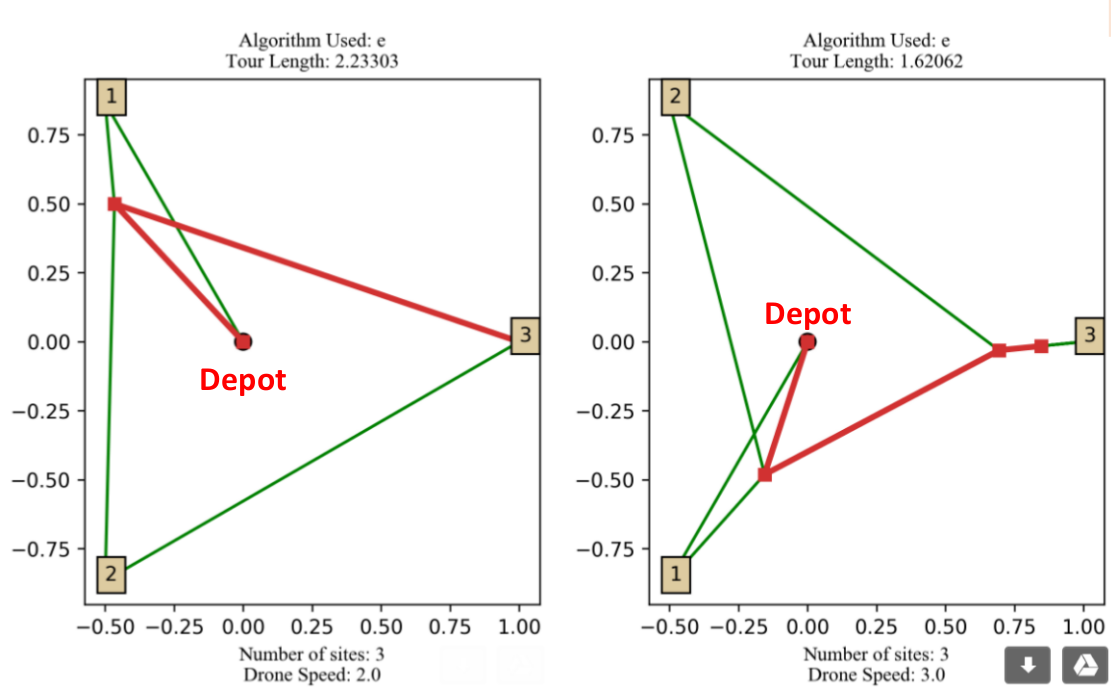
\includegraphics[width=10cm]{slide_imgs/drone_path_self_intersect.png}
  \end{figure}
\definecolor{byzantine}{rgb}{0.74, 0.2, 0.64}

\begin{center}
   {\color{byzantine} Unsure: Might the opt truck route self-intersect? We have not seen it,
    but exchange argument not yet working to prove it}
\end{center}

\end{frame}

%%%%%%%%%%%%%%%%%%%%%%%%%%%%%%%%%%%%%%%%%%%%%%%%%%%%%%%%%%%%%%%%%%%%%%%%%%%%%%%%%%%%%%%%%%%%%%%%%%
\begin{frame}{When Order of Visitation is Given (Exact Solution $L2$)}
  \vspace{-14pt}
  \begin{figure}[H]
    \centering
    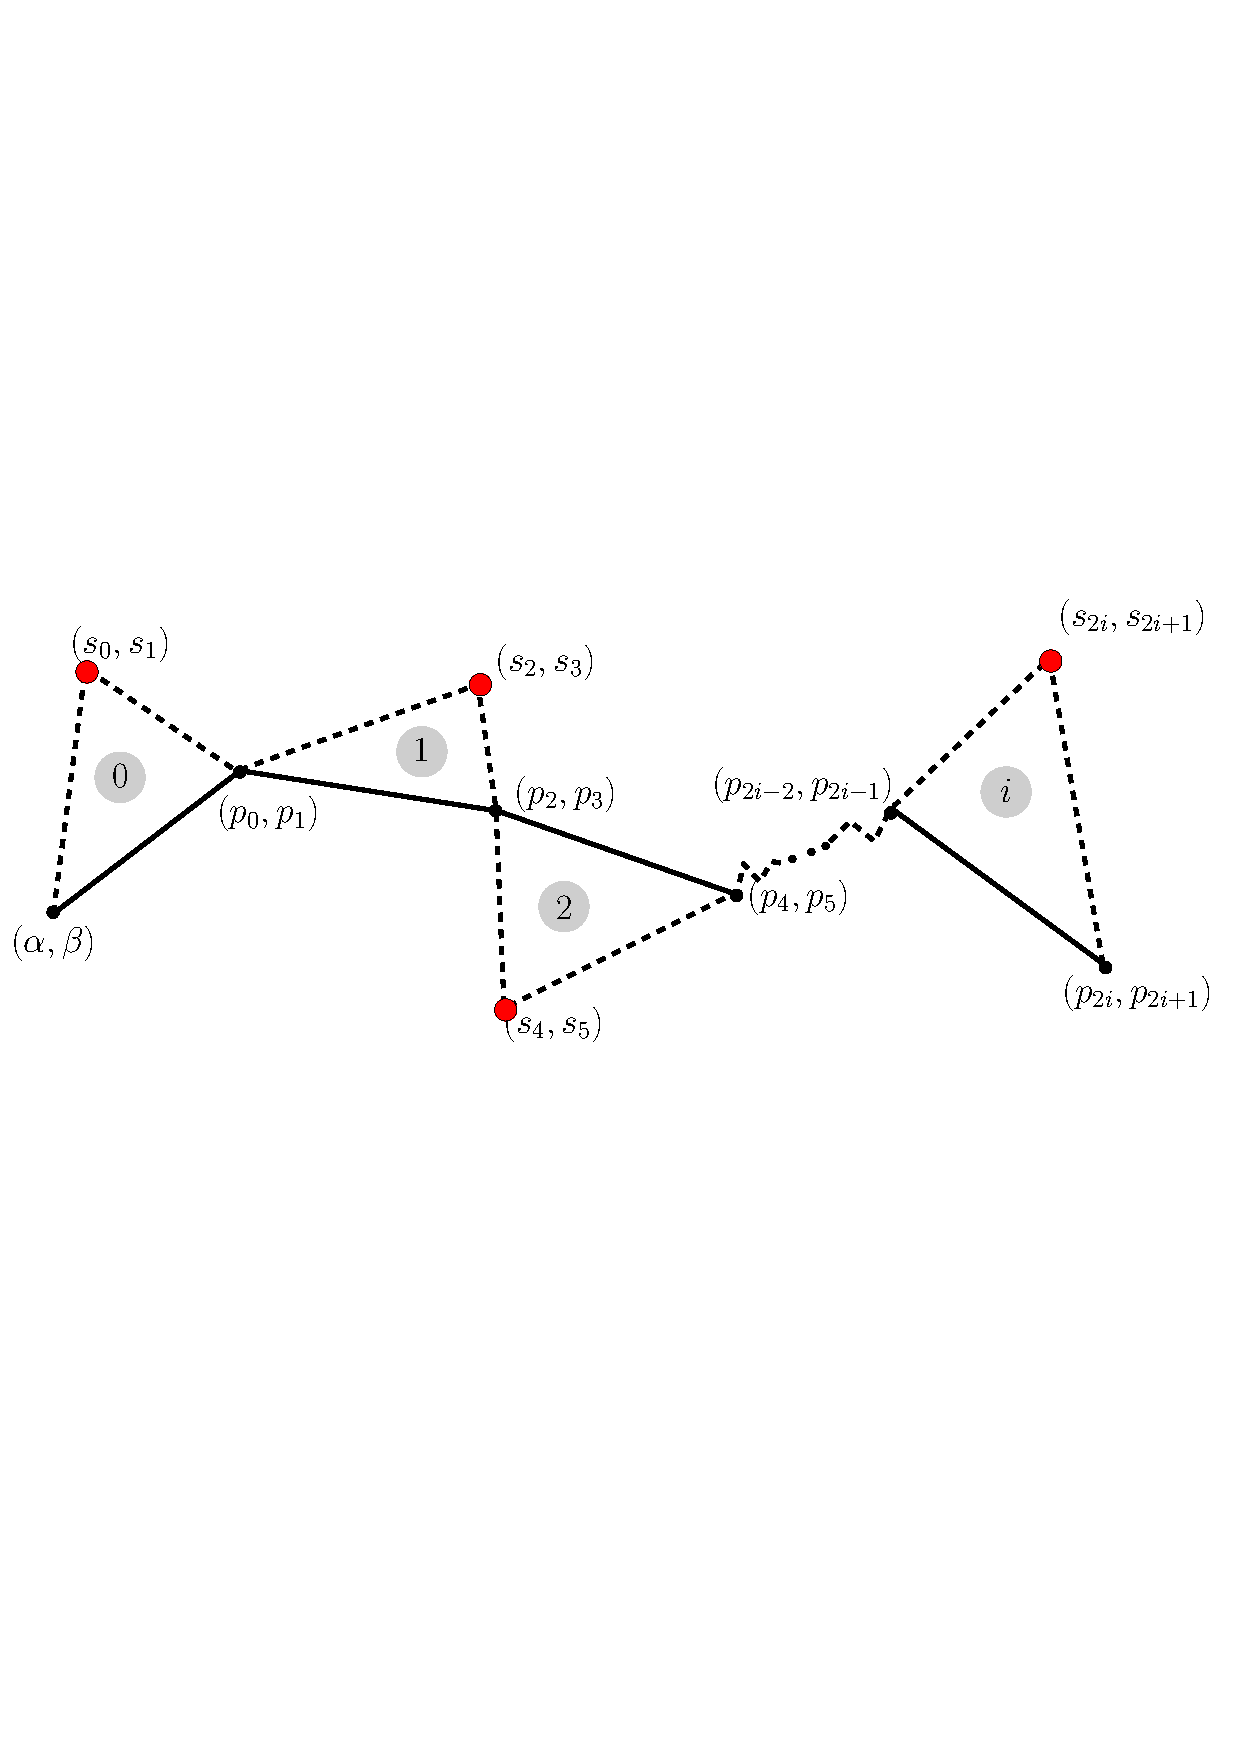
\includegraphics[width=10.5cm]{../img/lpdescr.pdf}
  \end{figure}
  \vspace{-10pt}
  \tiny{$$\displaystyle \min_{(p_0,p_1,\ldots,p_{2n-1}) \in \mathbb{R}^{2n}}  \sum_{i=1}^{n}  || P_i - P_{i-1} ||_2$$}

\vspace{-7pt}
subject to \(n\) constraints \\

\hspace{40pt}$||P_{i}-P_{i-1}||_2=\frac{ || P_{i-1}-S_{i}||_2 + ||S_{i}-P_{i}||_2}{\varphi}\qquad \text{for} \;\; i \in \{1,2,\ldots n\}$

 \begin{center}
     \definecolor{byzantine}{rgb}{0.74, 0.2, 0.64}
     \large {\color{byzantine} This can be formulated as an SOCP (Carlsson, Song), but in experiments here we use a generic non-linear solver from SciPy. } \normalsize
  \end{center}


\end{frame}

%%%%%%%%%%%%%%%%%%%%%%%%%%%%%%%%%%%%%%%%%%%%%%%%%%%%%%%%%%%%%%%%%%%%%%%%%%%%%%%%%%%%%%%%%%%%%%%%%%

\begin{frame}{When Order of Visitation is Given (Exact Solution $L1$)}
  \vspace{-12pt}
  \begin{figure}[H]
    \centering
    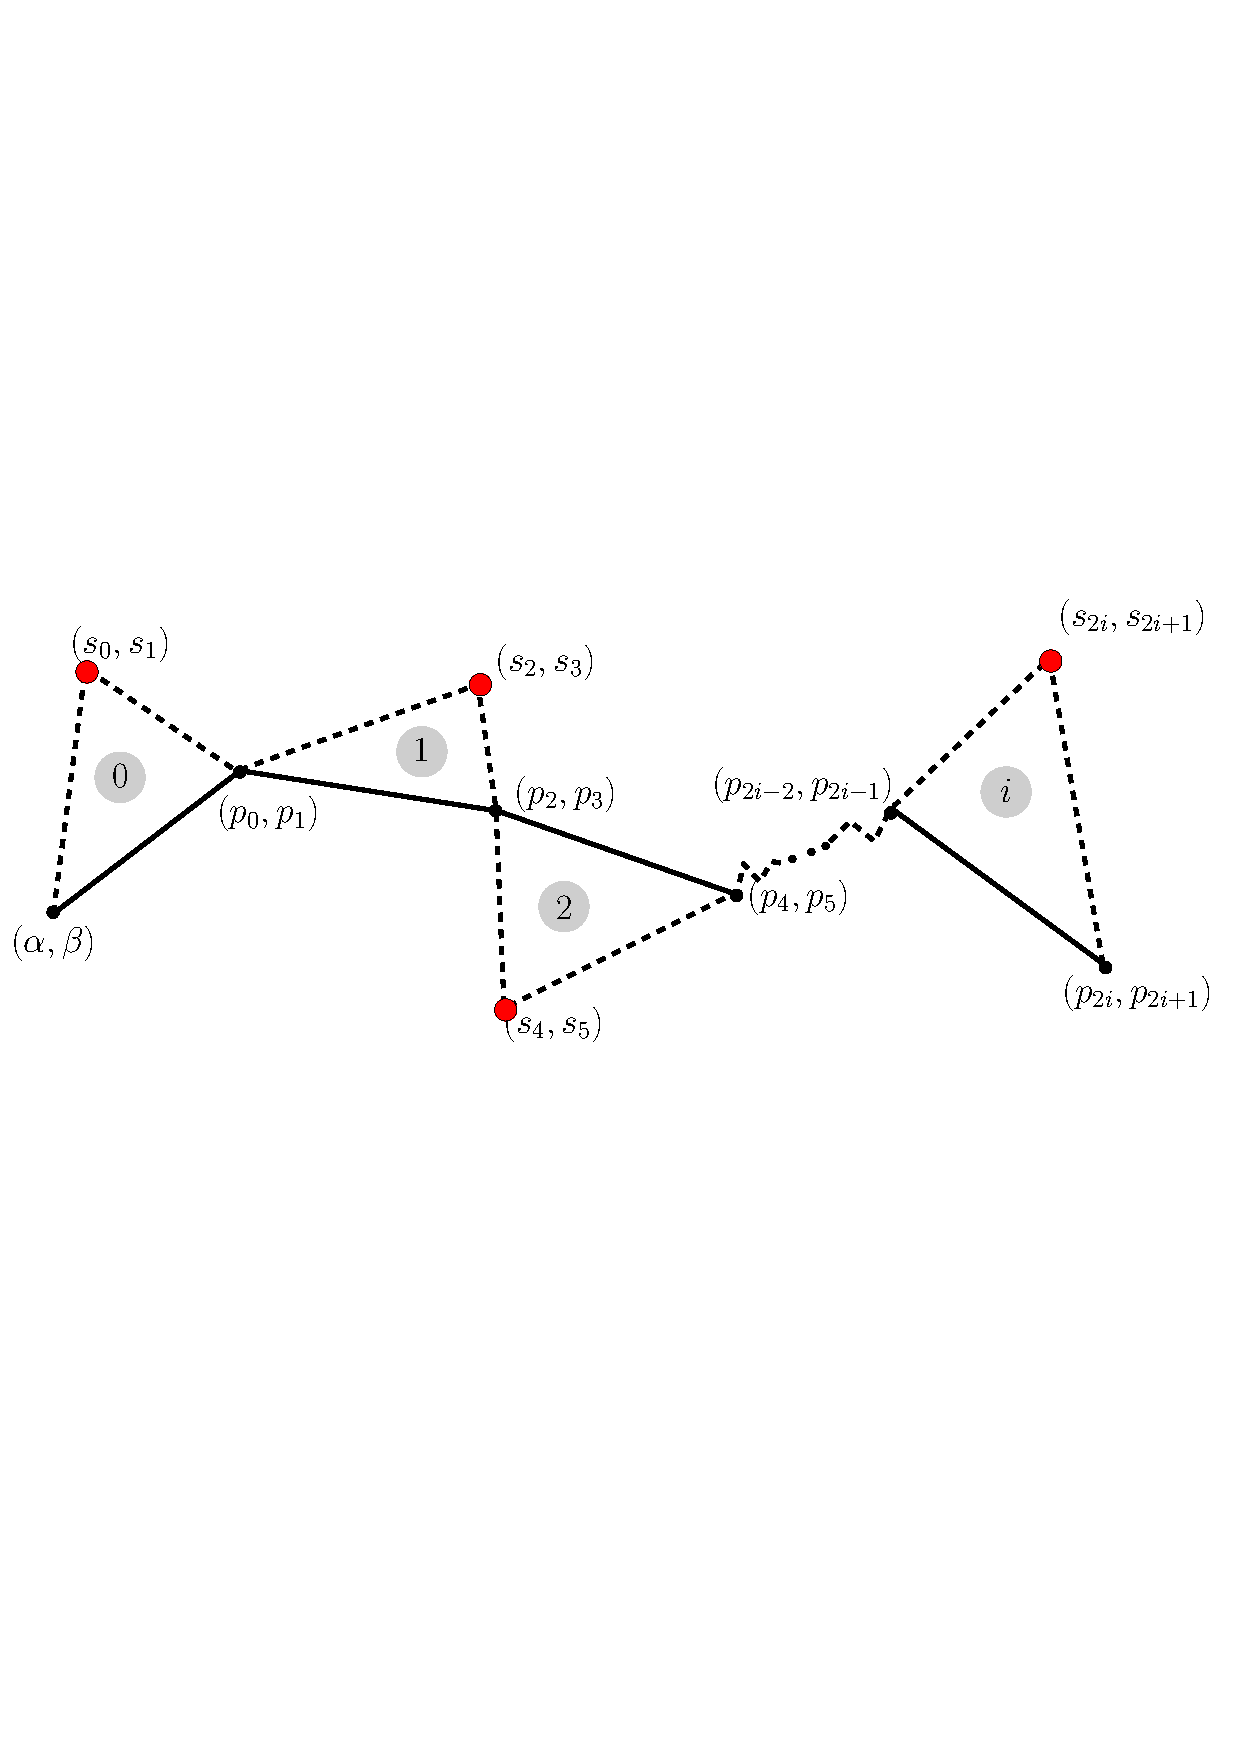
\includegraphics[width=8.0cm]{../img/lpdescr.pdf}
  \end{figure}
  \vspace{-10pt}
\tiny{  $$\displaystyle \min_{(p_0,p_1,\ldots,p_{2n-1}) \in \mathbb{R}^{2n}}  \sum_{i=1}^{n}  || P_i - P_{i-1} ||_1$$}

\vspace{-7pt}

\only<1>{
  \tiny{subject to \(n\) constraints }\\
  \tiny{\hspace{40pt}$||P_{i}-P_{i-1}||_1=\frac{ || P_{i-1}-S_{i}||_1 + ||S_{i}-P_{i}||_1}{\varphi}\qquad \text{for} \;\; i \in \{1,2,\ldots n\}$}
 \begin{center}
     \definecolor{byzantine}{rgb}{0.74, 0.2, 0.64}
     \large {\color{byzantine} This can be formulated as an LP. We use the MOSEK LP solver in our experiments.} \normalsize
  \end{center}


}

\only<2>{ \begin{columns}
    \begin{column} {0.5\textwidth}
      \begin{figure}
        \centering
        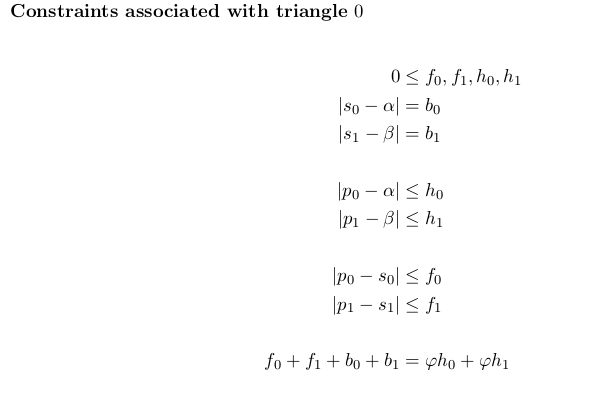
\includegraphics[width=5.9cm]{slide_imgs/tr0.png}
      \end{figure}
     \end{column}

    \begin{column}{0.5\textwidth}
      \begin{figure}
        \centering
        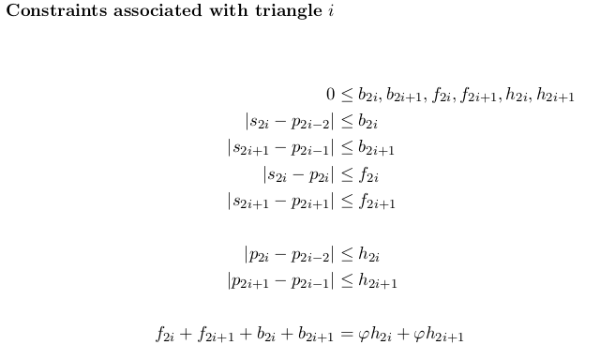
\includegraphics[width=5.9cm]{slide_imgs/tri.png}
      \end{figure}
     \end{column}
\end{columns}}



\end{frame}

\begin{frame}[t]{$L2$ Solution vs. $L1$ Solution: An Example}

  \vspace{-15pt}
  \begin{columns}
    \begin{column} {0.5\textwidth}
      \begin{center}
        Tour Length: 3.06500
      \end{center}
      \vspace{-20pt}
      \begin{figure}
        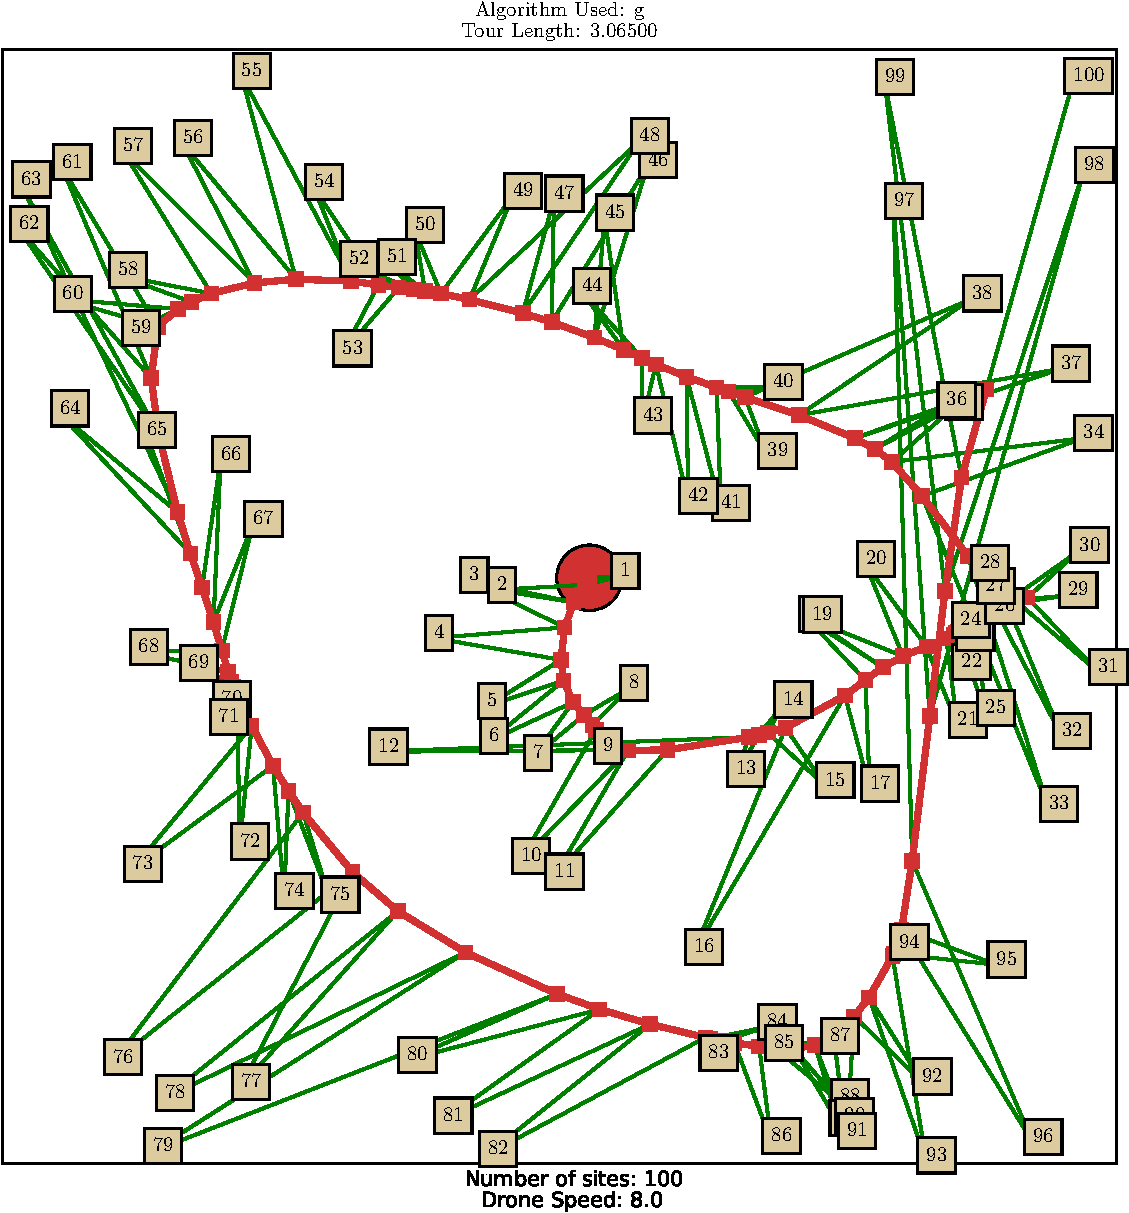
\includegraphics[width=5.4cm]{../img/Greedy_SLSQP.pdf}
      \end{figure}
     \end{column}

    \begin{column}{0.5\textwidth}
      \begin{center}
        Tour Length: 4.21343  
      \end{center}
      
      \vspace{-20pt}
       \begin{figure}
        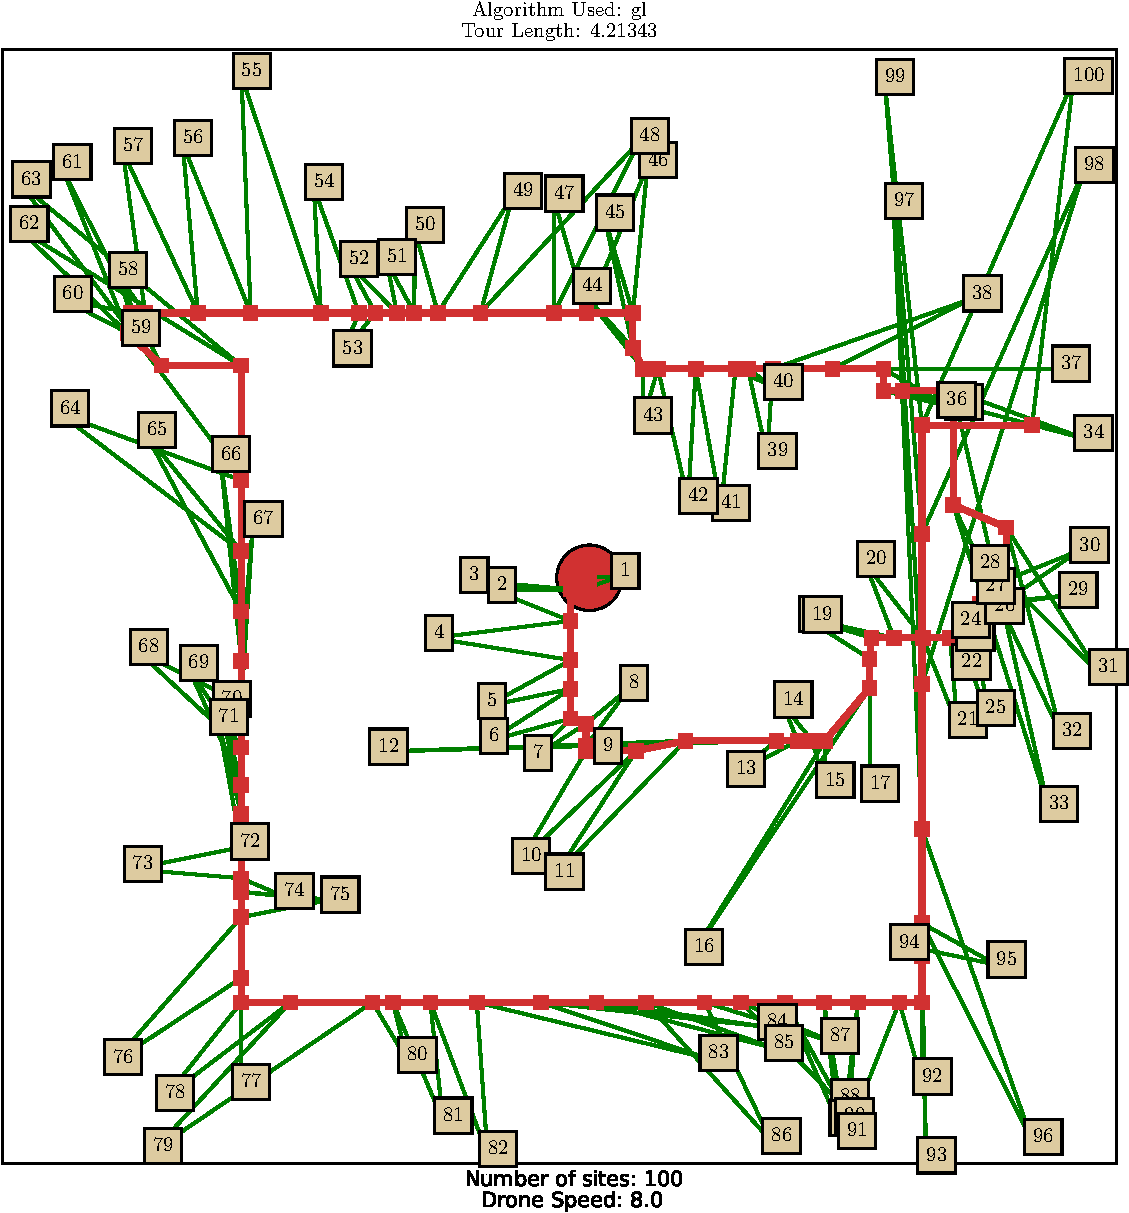
\includegraphics[width=5.4cm]{../img/Greedy_LP.pdf}
      \end{figure}
     \end{column}
   \end{columns}

   \vspace{-12pt}
   \begin{center}
     Number of Sites  = 100 \\
     \varphi          = 8.0 \\
       \small {Orderings of sites for both pictures are the \underline{same}. \\ Computed with a Greedy heuristic.} \normalsize
   \end{center}
   
   
\end{frame}

%%%%%%%%%%%%%%%%%%%%%%%%%%%%%%%%%%%%%%%%%%%%%%%%%%%%%%%%%%%%%%%%%%%%%%%%%%%%%%%%%%%%%%%%%%%%%%%%%%

\begin{frame}{$L2$ Solution vs. $L1$ Solution}
  \begin{figure}
        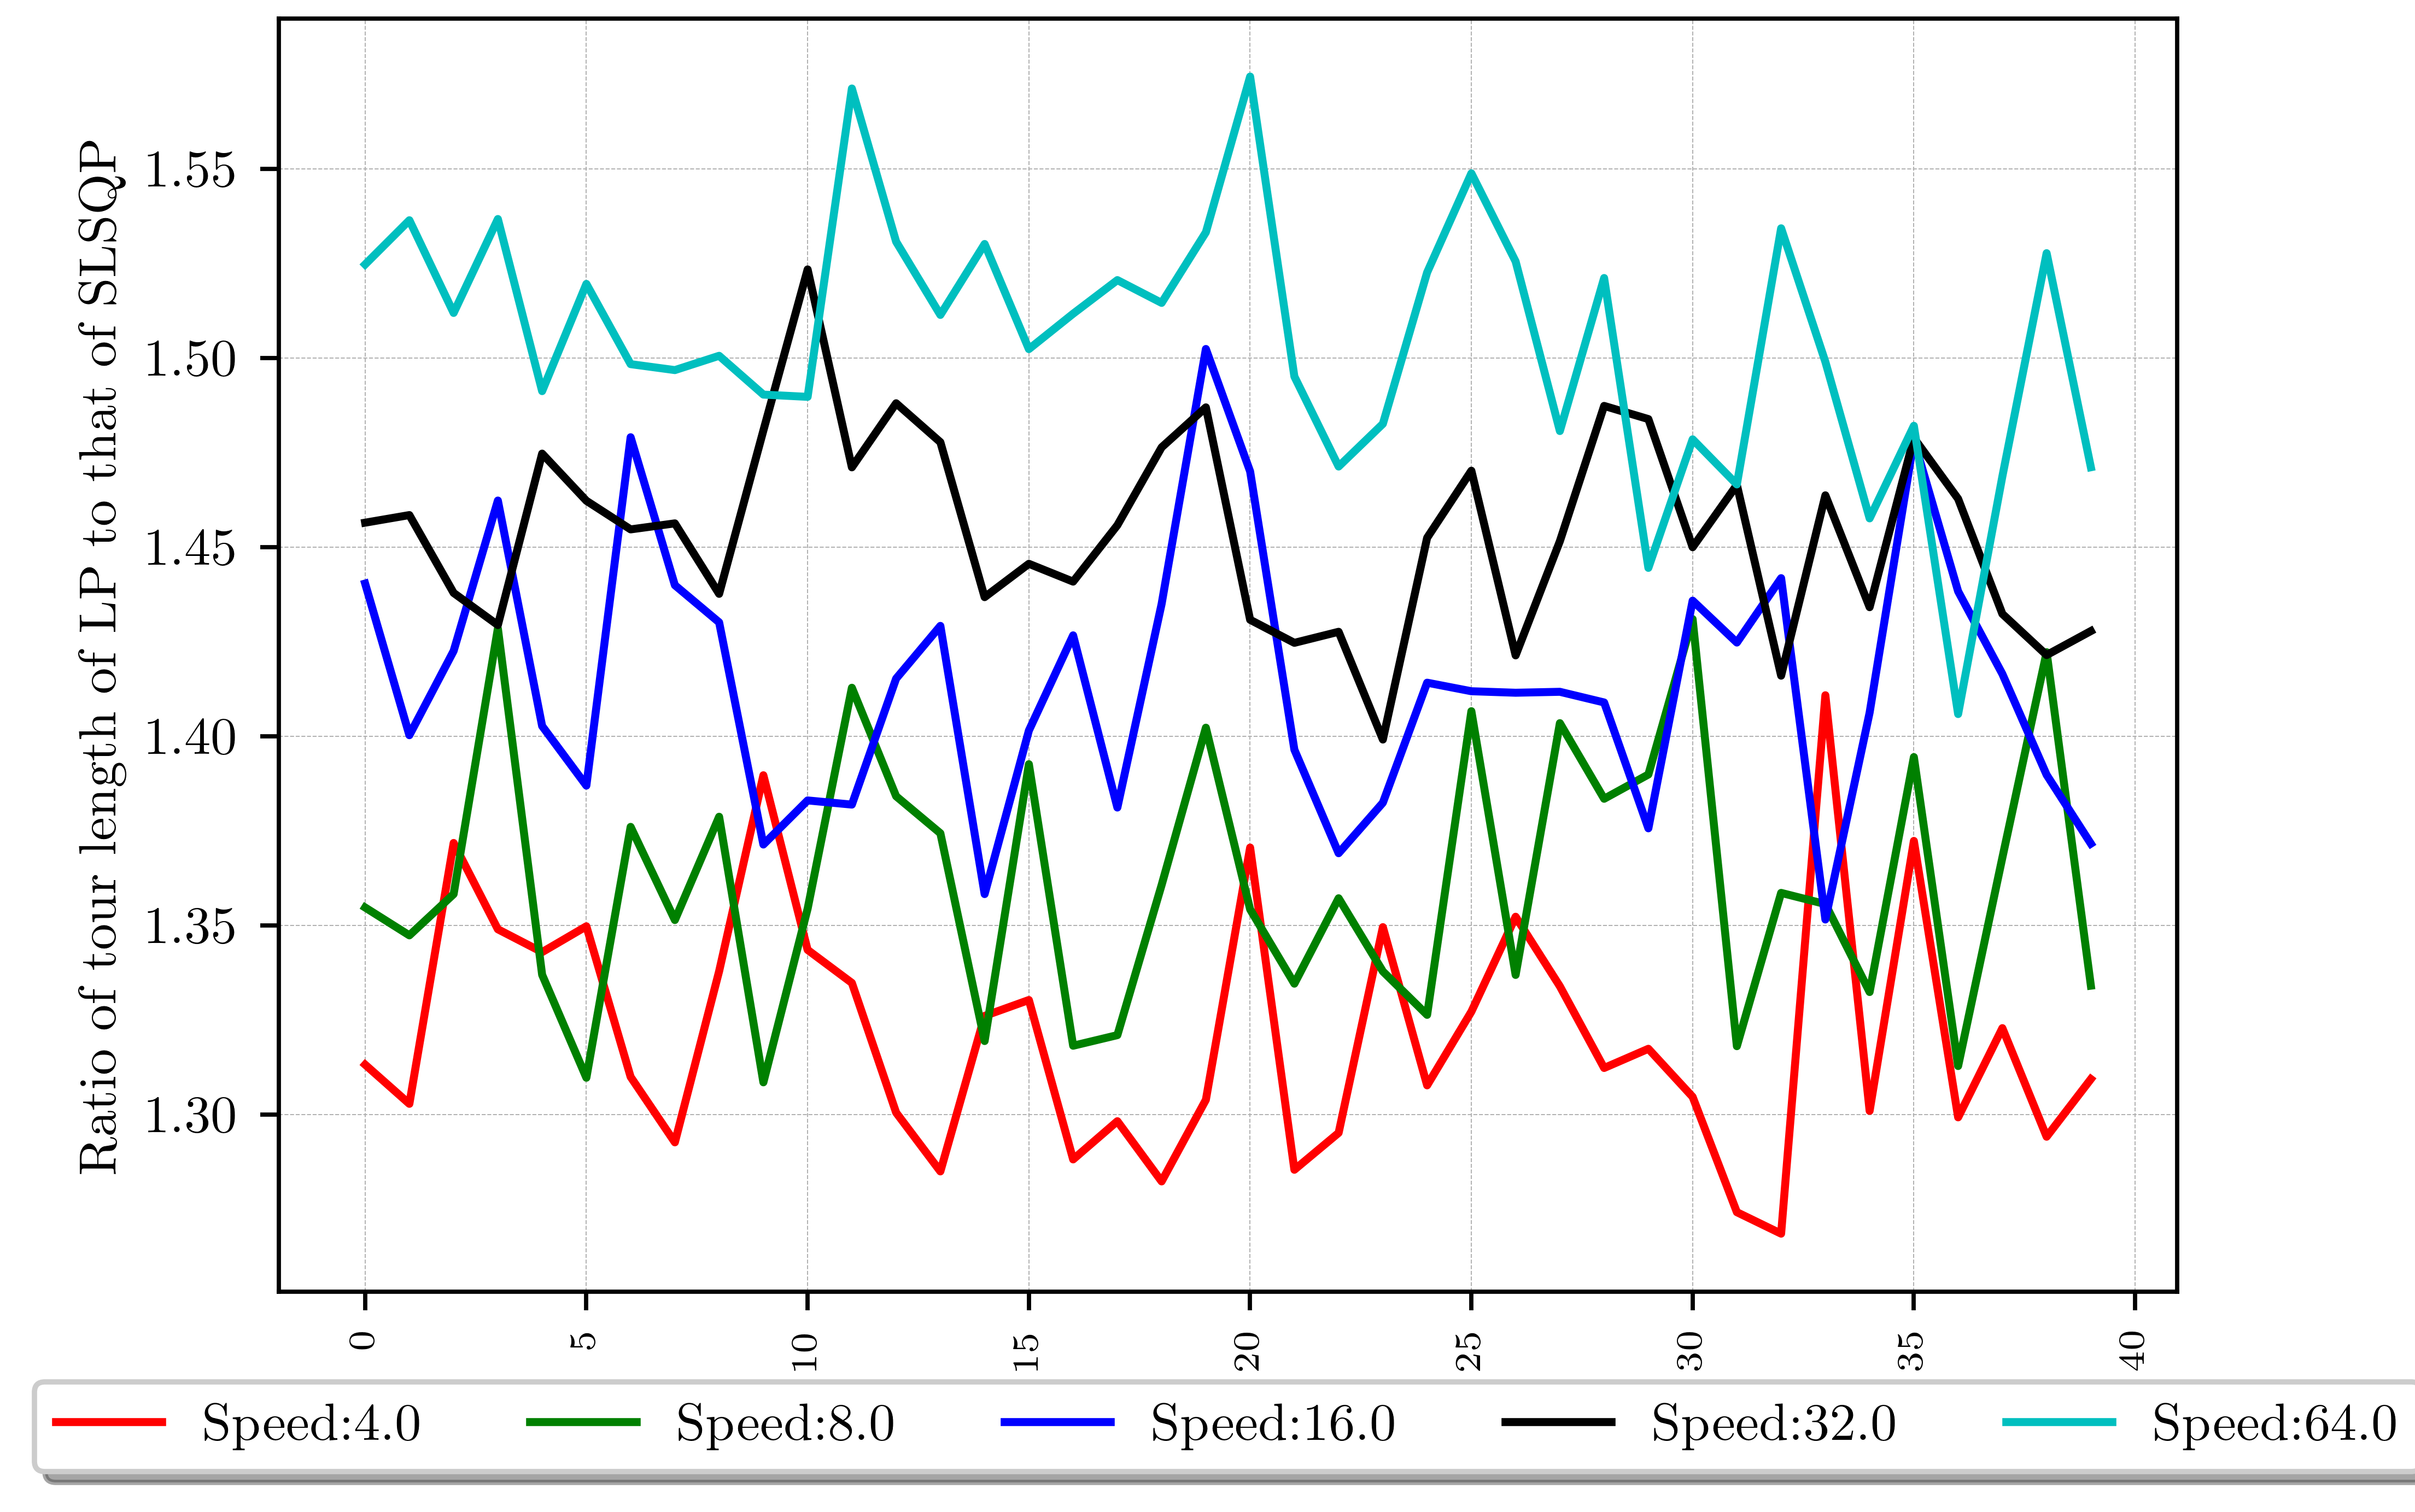
\includegraphics[width=10.0cm]{../img/tour_length_ratios.png}
        \caption*{Conjectured Worst-case Approximation Ratio of $L2$ to $L1$: {$\sqrt{2} \; o(\varphi) $}}
  \end{figure}
\end{frame}

%%%%%%%%%%%%%%%%%%%%%%%%%%%%%%%%%%%%%%%%%%%%%%%%%%%%%%%%%%%%%%%%%%%%%%%%%%%%%%%%%%%%%%%%%%%%%%%%%%

\begin{frame}{A Special Case: Collinear Horseflies}

  \begin{columns}
     \begin{column}{0.6\textwidth}

       \begin{figure}[H]
         \centering
         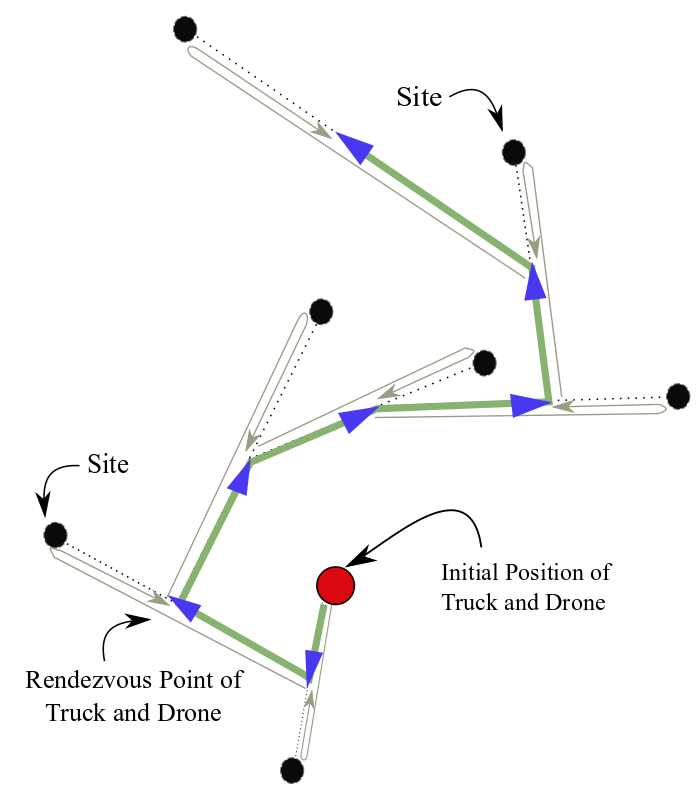
\includegraphics[width=6.0cm]{slide_imgs/collinear_horseflies.png}
       \end{figure}
       
     \end{column}
          
     \begin{column}{0.4\textwidth}
       \begin{center}
          \begin{framed}
             Truck and drone always move towards a site. 
           \end{framed}
        \end{center}
     \end{column}
  \end{columns}


  

\end{frame}

%%%%%%%%%%%%%%%%%%%%%%%%%%%%%%%%%%%%%%%%%%%%%%%%%%%%%%%%%%%%%%%%%%%%%%%%%%%%%%%%%%%%%%%%%%%%%%%%%%
\begin{frame}{Greedy Heuristic (1) : Nearest Neighbor }

  \begin{columns}
    \begin{column}{0.6\textwidth}
      \begin{figure}[H]
        \centering
        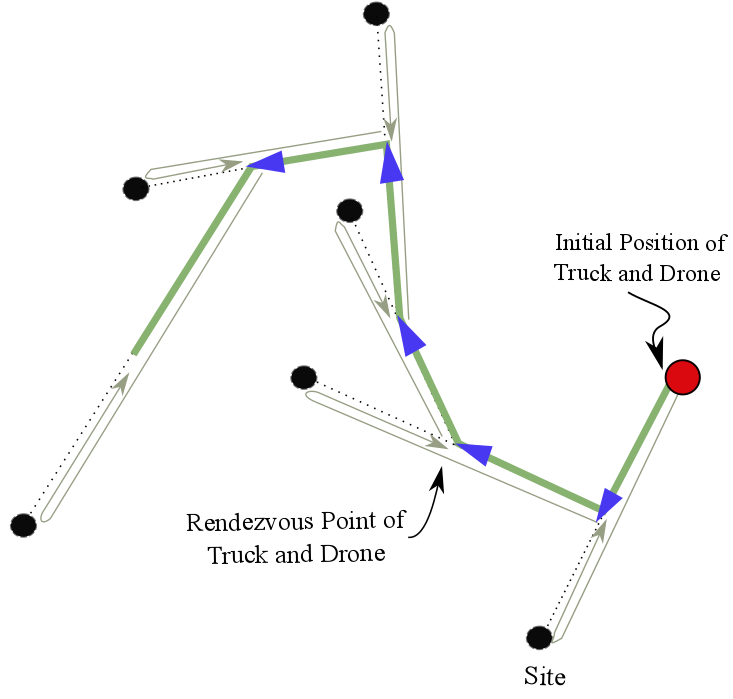
\includegraphics[width=6.6cm]{slide_imgs/nearest_unvisited_neighbor.png}
      \end{figure}
     \end{column}
    
    \begin{column}{0.4\textwidth}
      \begin{center}
        \begin{framed}
          Truck and drone visit the nearest unserviced site. 
        \end{framed}
      \end{center}
    \end{column}
  \end{columns}


  \end{frame}

%%%%%%%%%%%%%%%%%%%%%%%%%%%%%%%%%%%%%%%%%%%%%%%%%%%%%%%%%%%%%%%%%%%%%%%%%%%%%%%%%%%%%%%%%%%%%%%%%%
\begin{frame}{Greedy Heuristic (2) : Cheapest Insertion }

  % https://stackoverflow.com/a/26189728
  % A very odd issue with Latex + Beamer which explains the strange
  % brace pattern below. 
  \begin{figure}[H]
    \centering
     \only<1>
      {%
      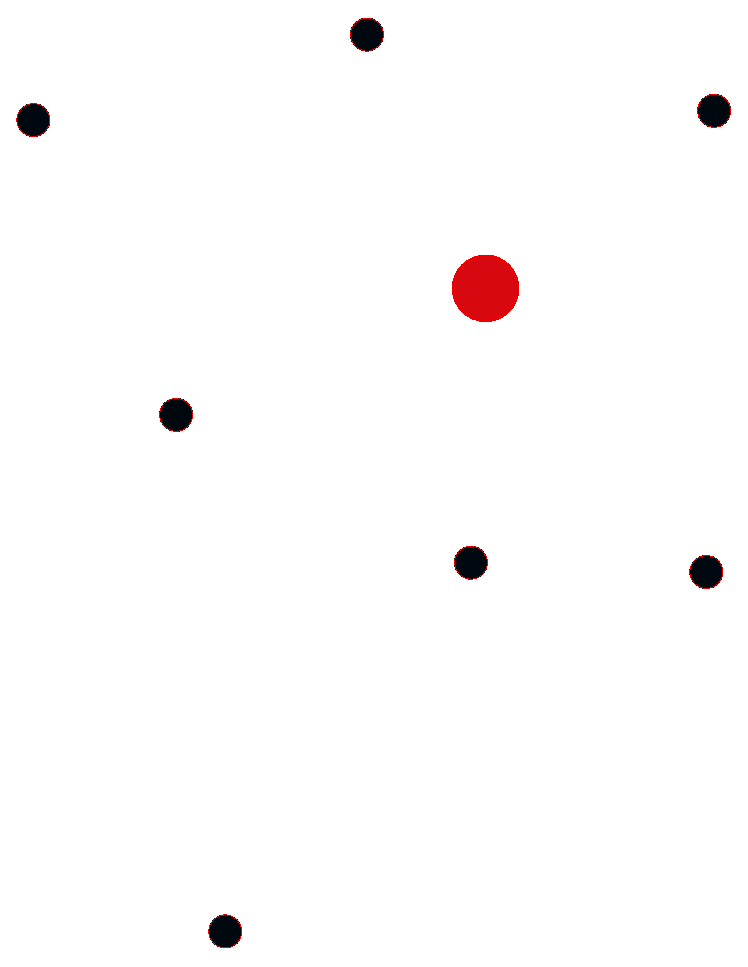
\includegraphics[width=4.5cm]{slide_imgs/input.eps}
      }%
      \only<2>
      {%
        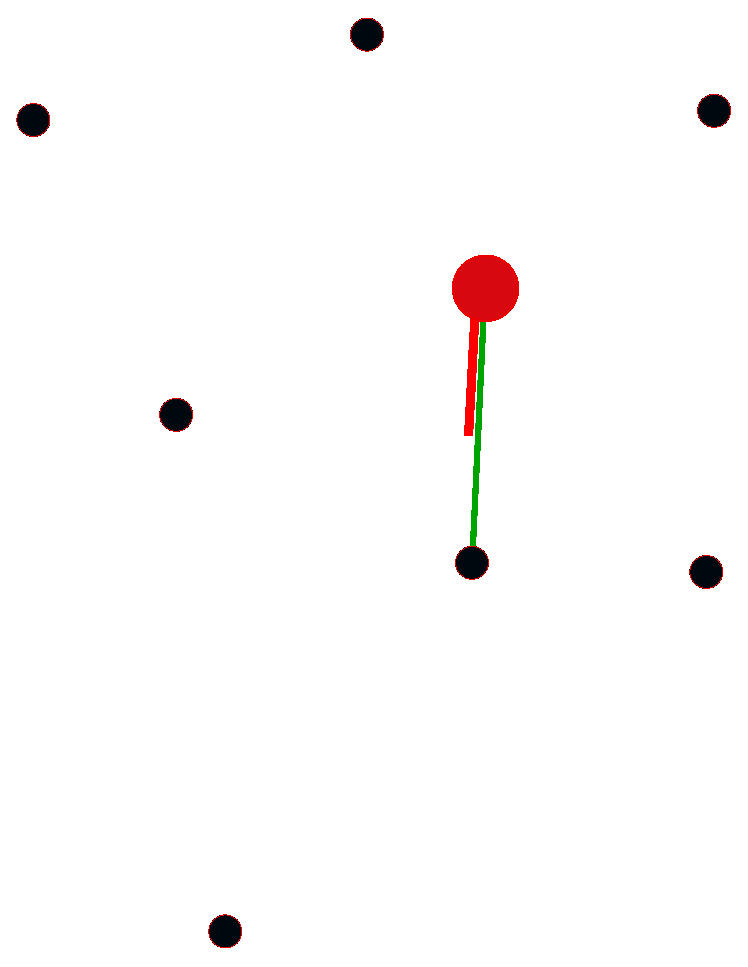
\includegraphics[width=4.5cm]{slide_imgs/point1.eps}
      }%
      \only<3>
      {%
        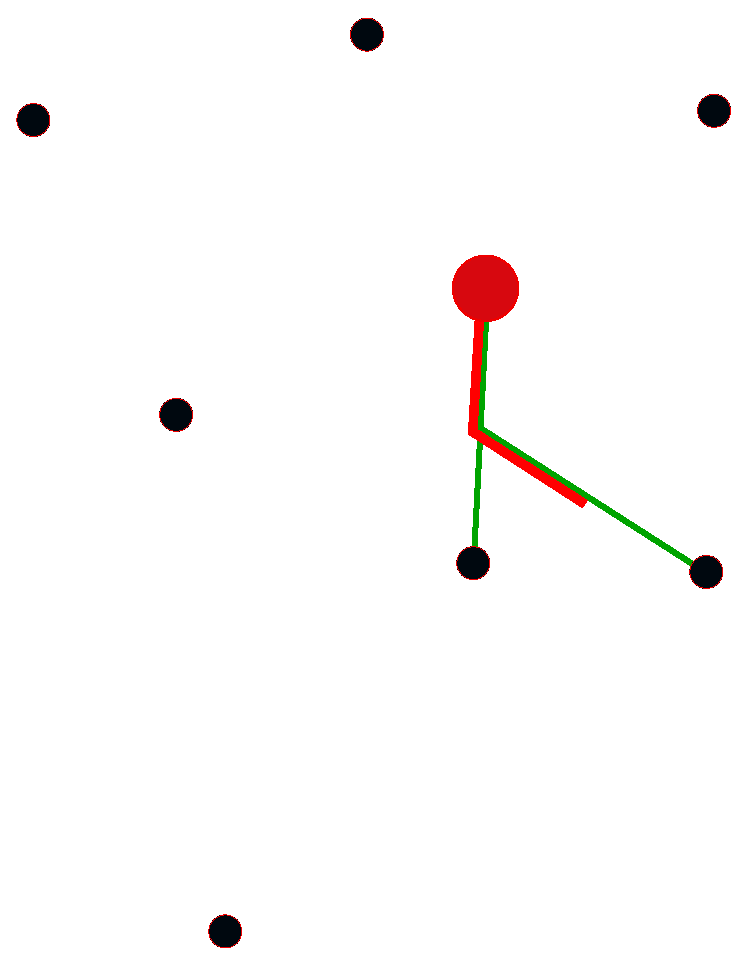
\includegraphics[width=4.5cm]{slide_imgs/point2.eps}
      }%

      \only<4>
      {%
        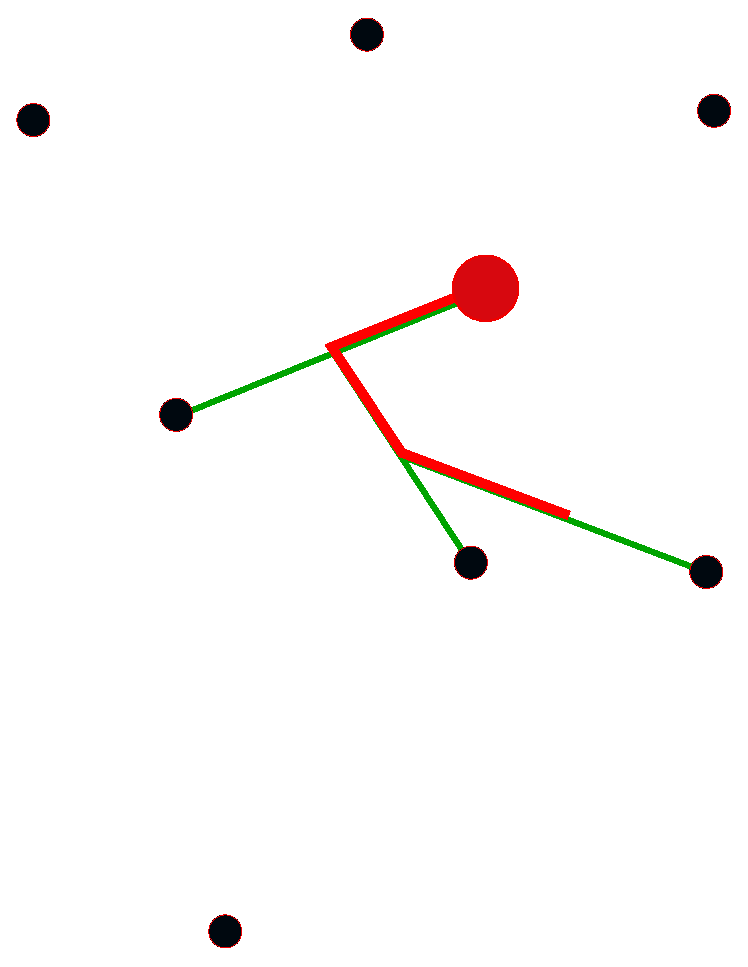
\includegraphics[width=4.5cm]{slide_imgs/point3.eps}
      }%

      \only<5>
      {%
        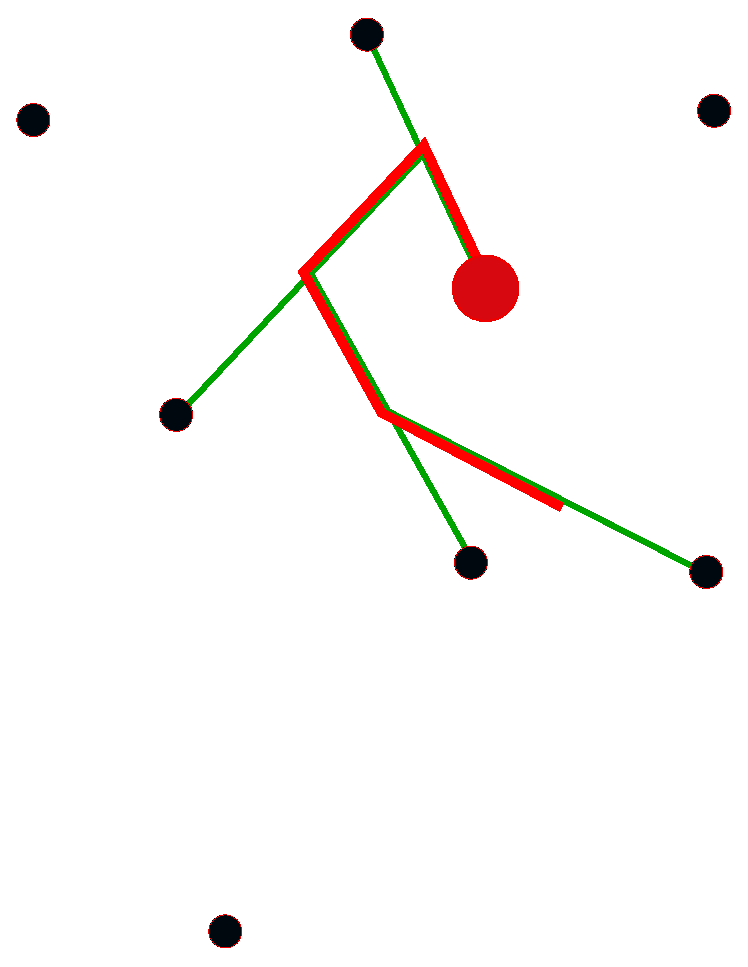
\includegraphics[width=4.5cm]{slide_imgs/point4.eps}
      }%
      \only<6>
      {%
        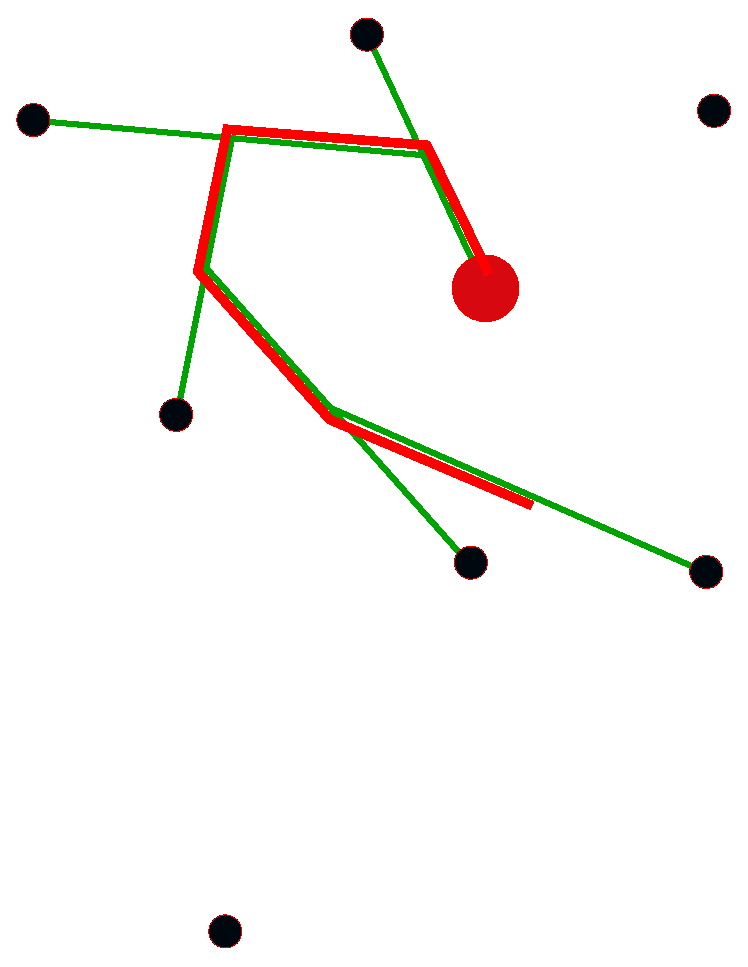
\includegraphics[width=4.5cm]{slide_imgs/point5.eps}
      }%
      \only<7>
      {%
        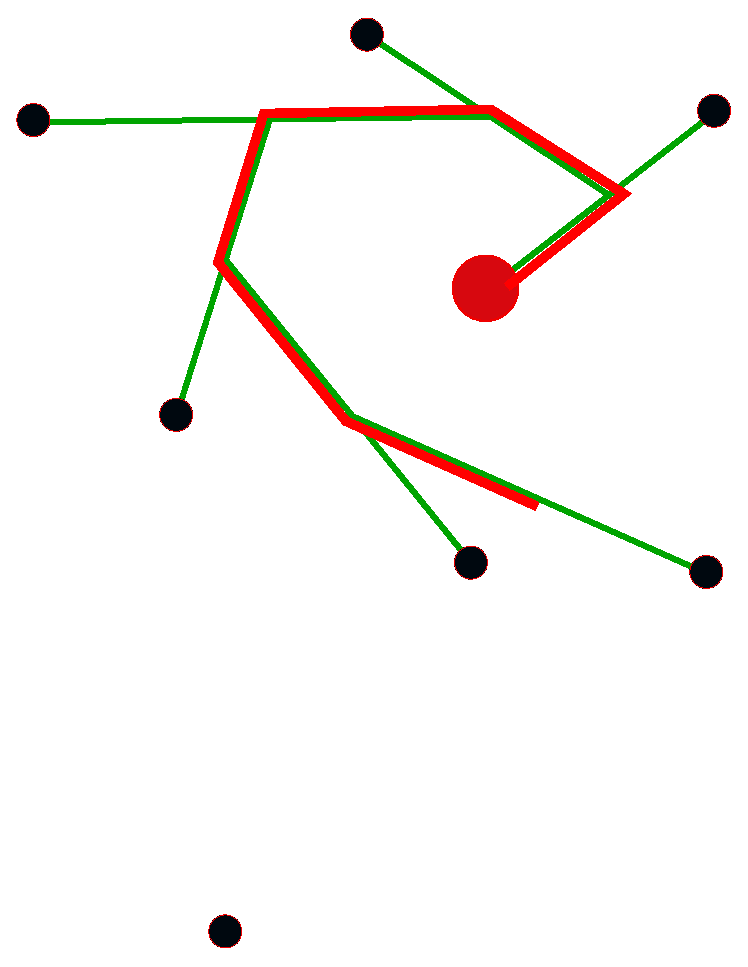
\includegraphics[width=4.5cm]{slide_imgs/point6.eps}
      }%
      \only<8>
      {%
        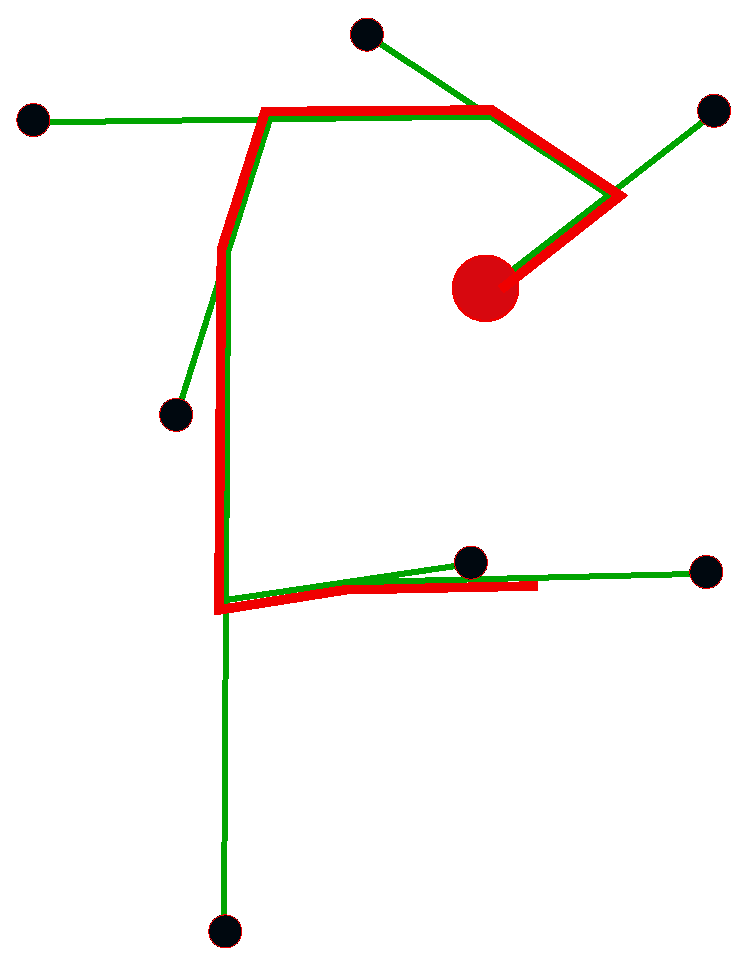
\includegraphics[width=4.5cm]{slide_imgs/point7.eps}
      }%

    
     \end{figure}
  \begin{center}

     \definecolor{byzantine}{rgb}{0.74, 0.2, 0.64}
     {\color{byzantine}In the case of TSP ($\varphi=1$), this strategy gives us a 2 approximation. \\

              Belief : For Horsefly the approximation is $ O(1) o(\varphi)$} \normalsize
  \end{center}
\end{frame}

%%%%%%%%%%%%%%%%%%%%%%%%%%%%%%%%%%%%%%%%%%%%%%%%%%%%%%%%%%%%%%%%%%%%%%%%%%%%%%%%%%%%%%%%%%%%%%%%%%
\begin{frame}{K2means Heuristic}
   \begin{figure}[H]
    \centering
    \only<1>{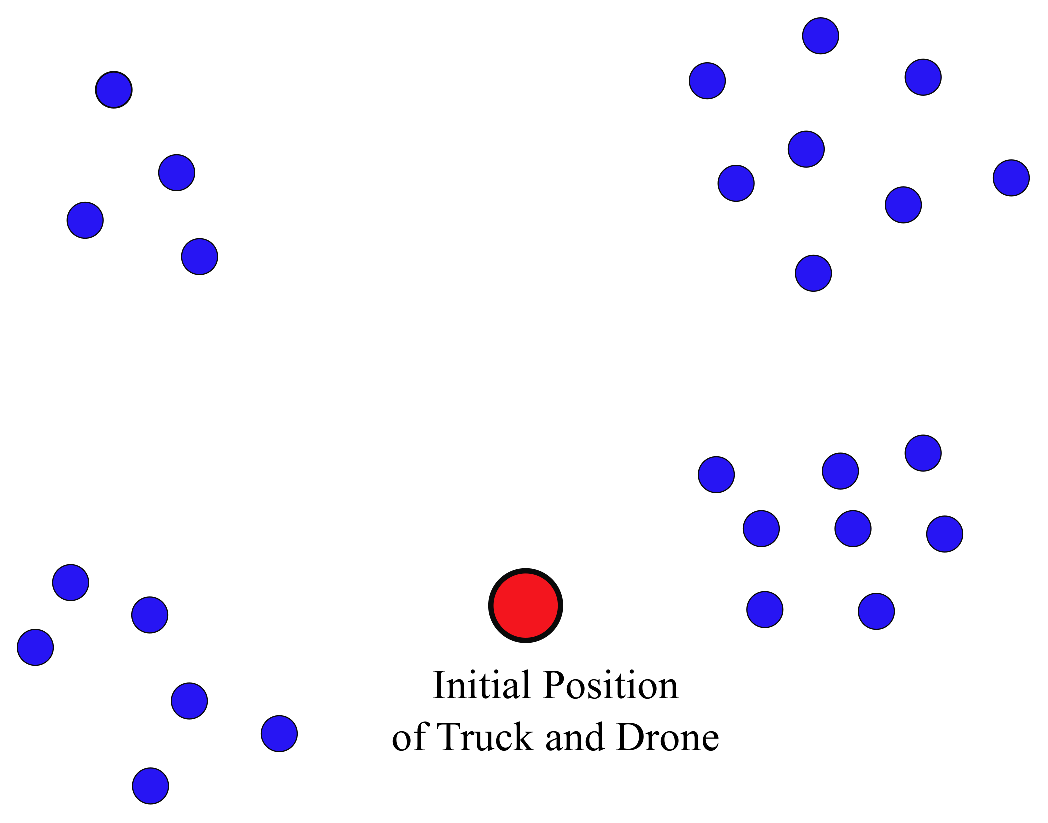
\includegraphics[width=6.6cm]{slide_imgs/k2means_explain_input.eps}}
    \only<2>{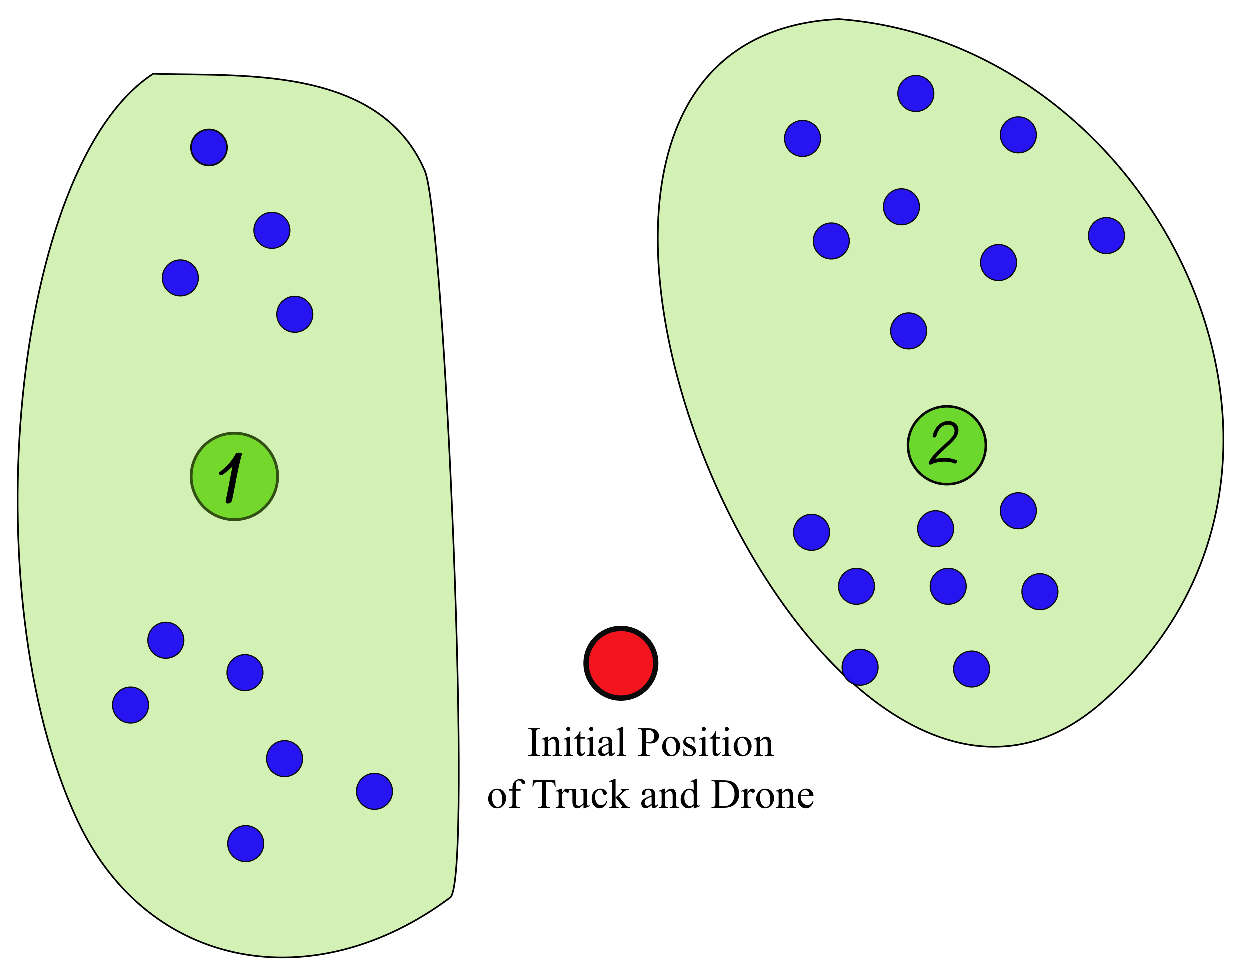
\includegraphics[width=8.0cm]{slide_imgs/k2means_explain_cluster1.eps}}
    \only<3>{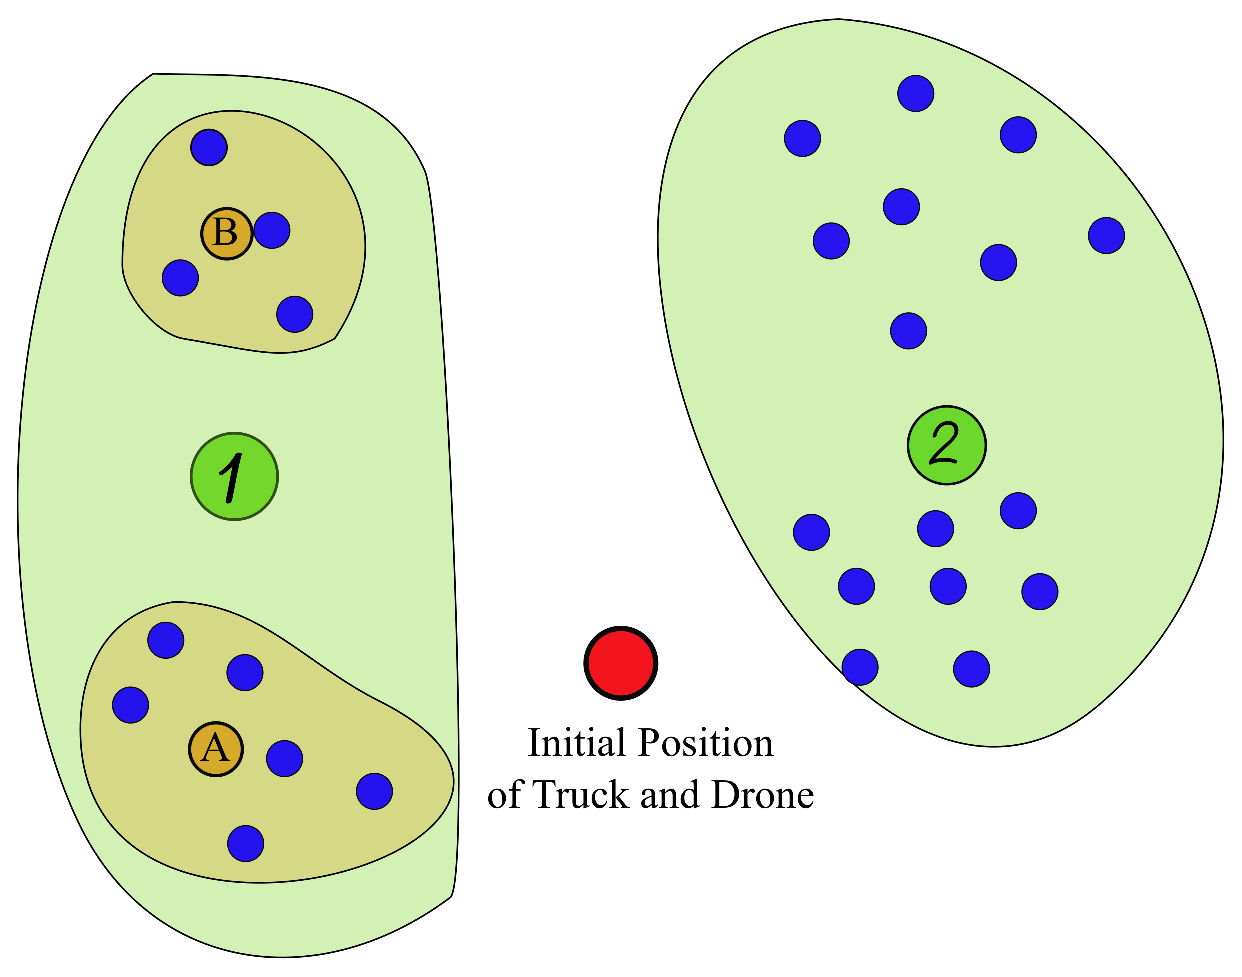
\includegraphics[width=8.0cm]{slide_imgs/k2means_explain_cluster2.eps}}
  \end{figure}
\end{frame}
%%%%%%%%%%%%%%%%%%%%%%%%%%%%%%%%%%%%%%%%%%%%%%%%%%%%%%%%%%%%%%%%%%%%%%%%%%%%%%%%%%%%%%%%%%%%%%%%%%
\begin{frame}{Comparing Nearest Neighbor and K2means heuristic}
 \begin{columns}
   \begin{column} {0.5\textwidth}
      \begin{center}
        Tour Length: 2.27952 \\
            Greedy (1)
      \end{center}
      \vspace{-20pt}

      \begin{figure}
        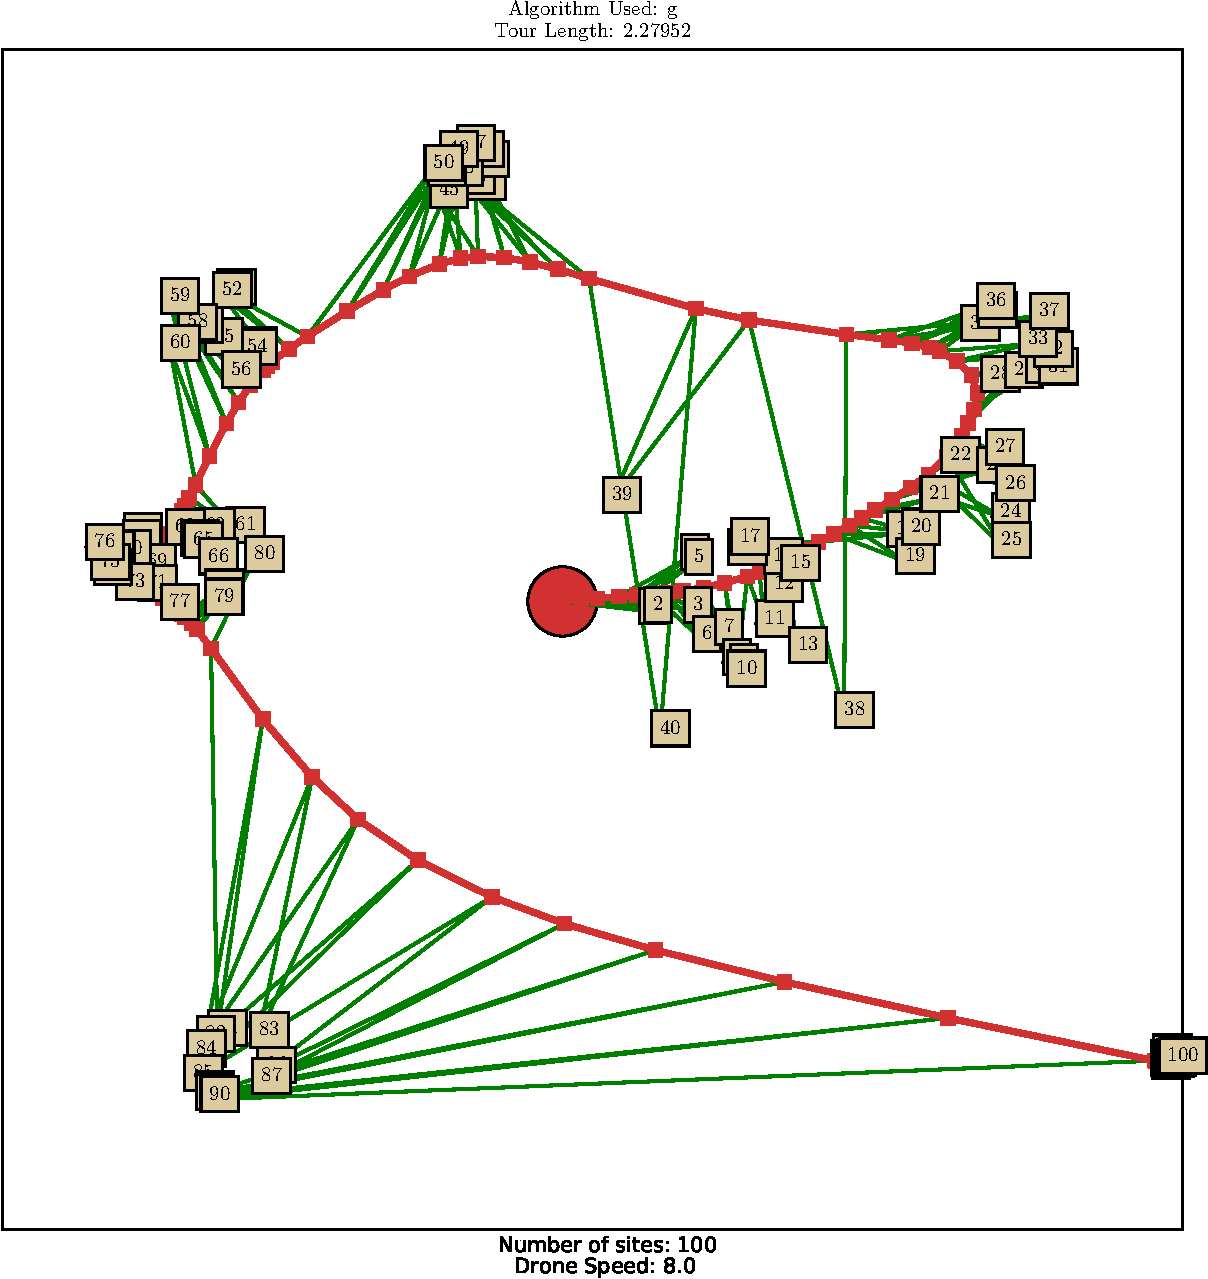
\includegraphics[width=5.2cm]{../img/greedy_example.pdf}
      \end{figure}
    \end{column}

    \begin{column}{0.5\textwidth}
            \begin{center}
              Tour Length: 3.06633 \\
                  K2means
      \end{center}

      \vspace{-20pt}
       \begin{figure}
        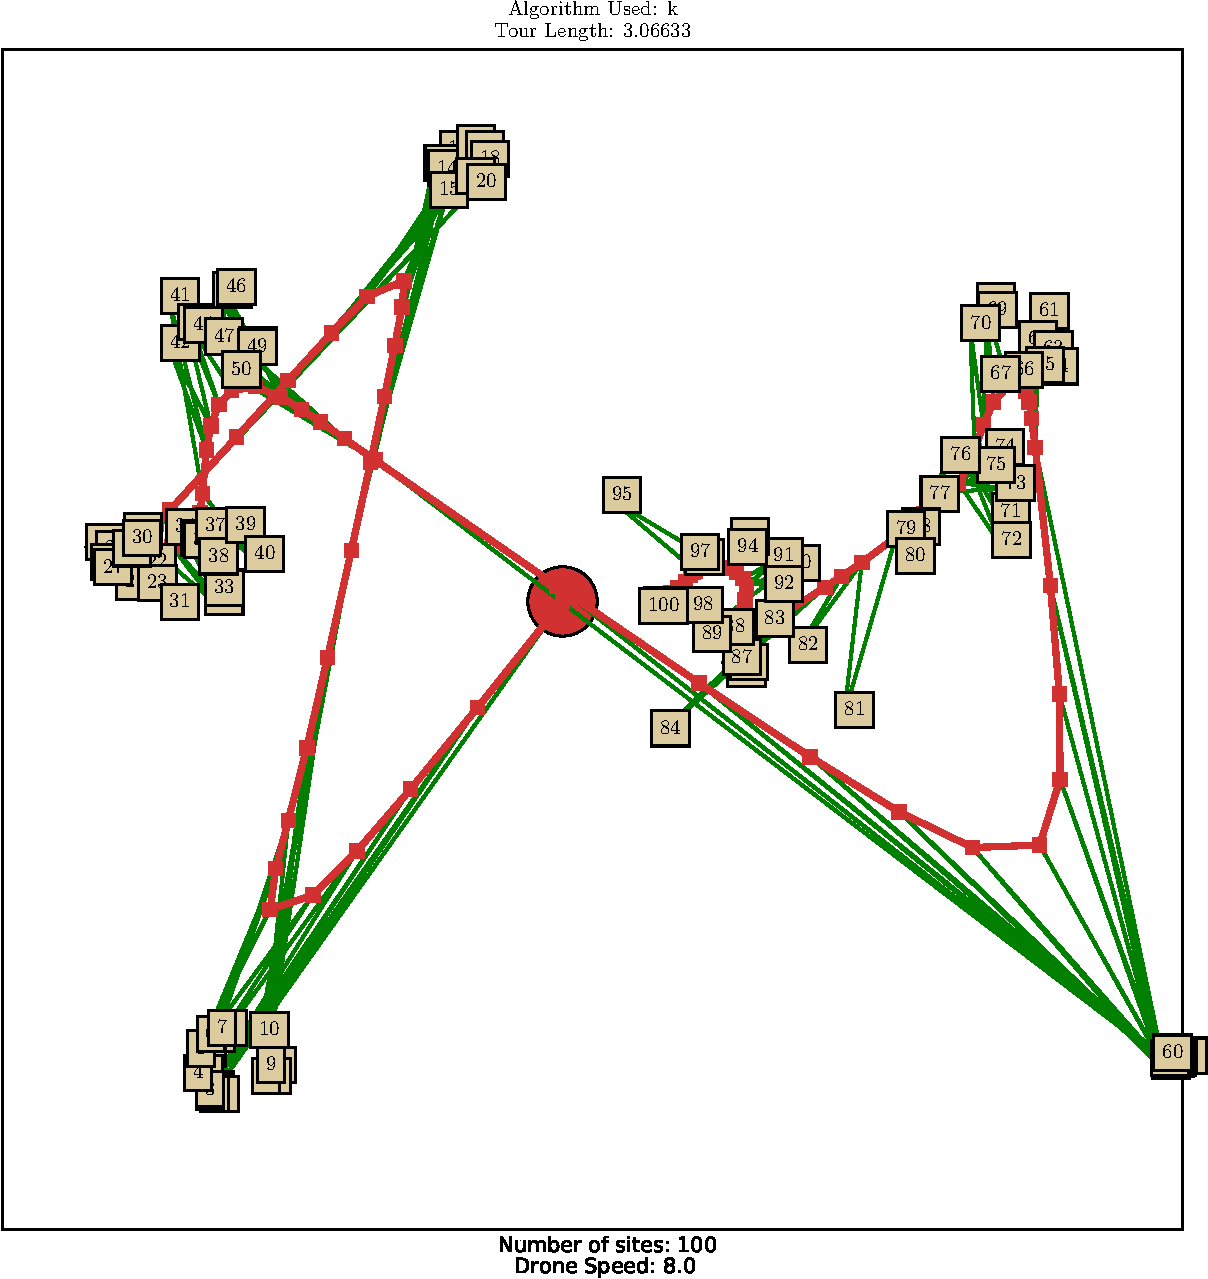
\includegraphics[width=5.2cm]{../img/k2means_example.pdf}
      \end{figure}
     \end{column}
   \end{columns}

   \begin{center}
     Number of Sites: 100 \\
     Drone Speed: 8.0
   \end{center}

\end{frame}

%%%%%%%%%%%%%%%%%%%%%%%%%%%%%%%%%%%%%%%%%%%%%%%%%%%%%%%%%%%%%%%%%%%%%%%%%%%
\begin{frame}[t]{Comparing Nearest Neighbor and K2means heuristic}
  \vspace{-20pt}
  \begin{figure}
    \centering
     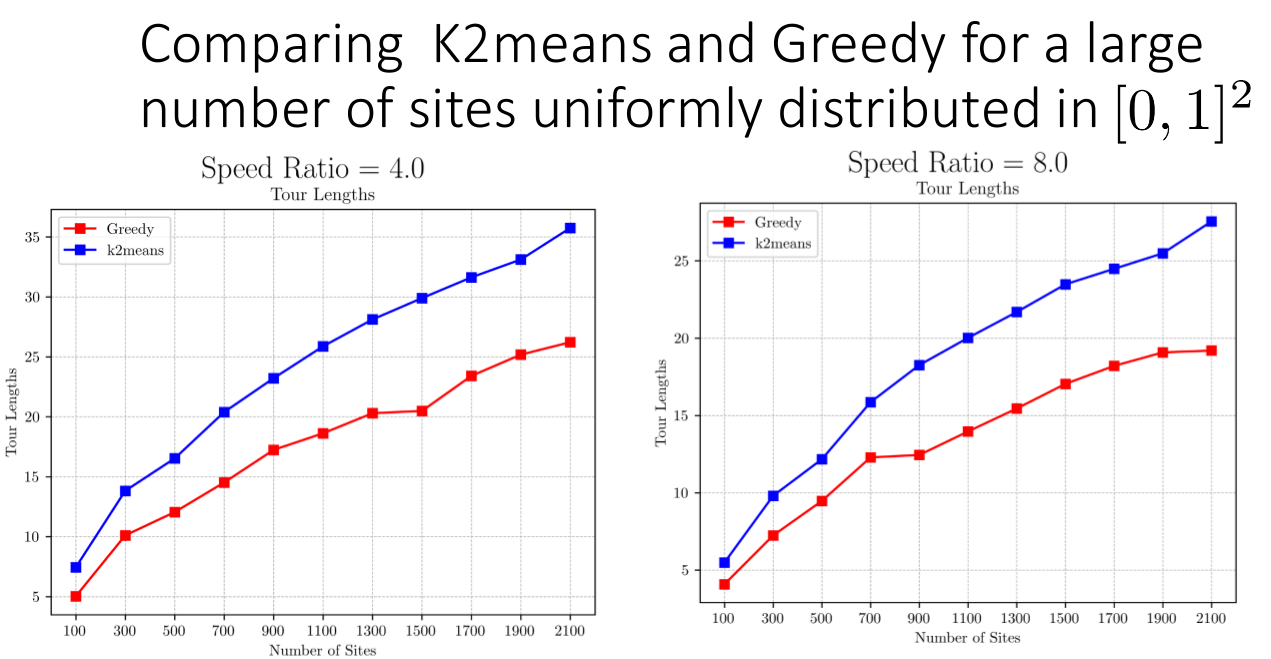
\includegraphics[width=12cm]{slide_imgs/compare_k2means_greedy.png}
   \end{figure}
\end{frame}


%%%%%%%%%%%%%%%%%%%%%%%%%%%%%%%%%%%%%%%%%%%%%%%%%%%%%%%%%%%%%%%%%%%%%%%%%%%
% Some heuristics and algorithms along
% with conjectured guarantees. Mention
% the scheme based on building trees
% bottom-up which works for arbitrary numbers
% of drones? 

\begin{frame}{An $O(\log n)$ approximation}

  \begin{figure}
        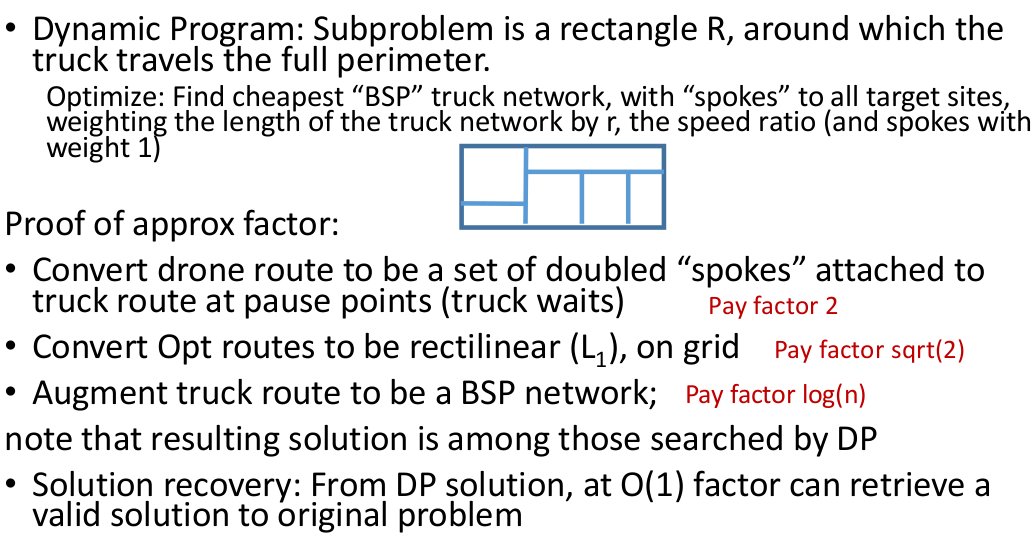
\includegraphics[width=10.0cm]{slide_imgs/logn_approx.png}
  \end{figure}

\end{frame}
%%%%%%%%%%%%%%%%%%%%%%%%%%%%%%%%%%%%%%%%%%%%%%%%%%%%%%%%%%%%%%%%%%%%%%%%%%%%

\begin{frame}{Weighted Backbone-and-Spoke Spanning Tree}

  \begin{figure}
        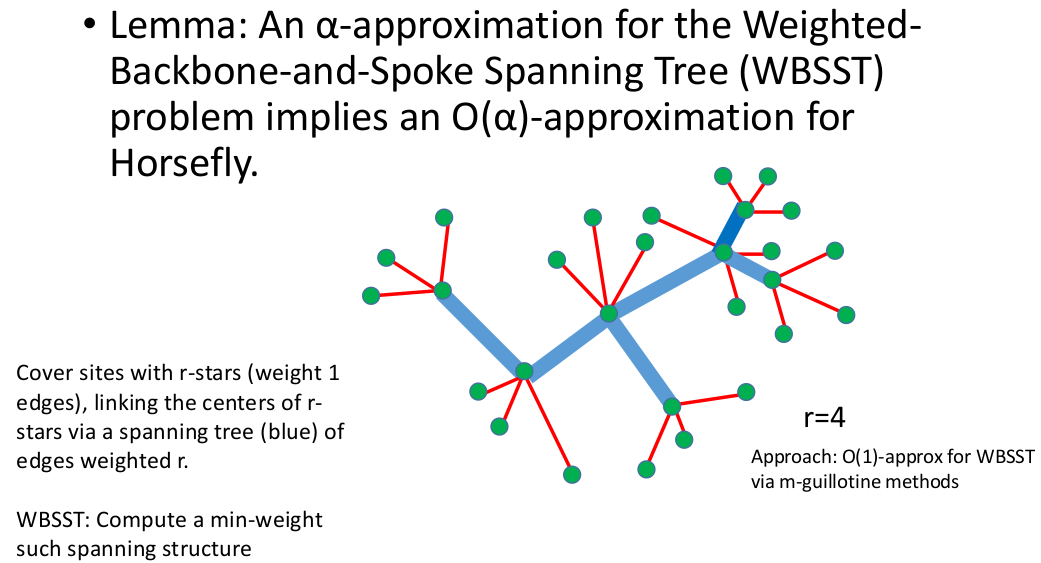
\includegraphics[width=10.0cm]{slide_imgs/wbsst.png}
  \end{figure}

\end{frame}


%%%%%%%%%%%%%%%%%%%%%%%%%%%%%%%%%%%%%%%%%%%%%%%%%%%%%%%%%%%%%%%%%%%%%%%%%%%%
\begin{frame}{Previous Work}
    \begin{itemize}
       \item \textbf{Coordinated logistics with a truck and a drone} \newline\textit{John Gunnar Carlsson, Siyuan Song} \newline Blah Blah
       \item \textbf{The flying sidekick traveling salesman problem: Optimization of drone-assisted parcel delivery} \newline \textit{Chase C.Murray, Amanda G.Chu} \newline \textit{Blah Blah}
    \end{itemize}
\end{frame}
%%%%%%%%%%%%%%%%%%%%%%%%%%%%%%%%%%%%%%%%%%%%%%%%%%%%%%%%%%%%%%%%%%%%%%%%%%%

\begin{frame}{Variants: Reverse Horsefly}
  \begin{figure}
    \centeringe
        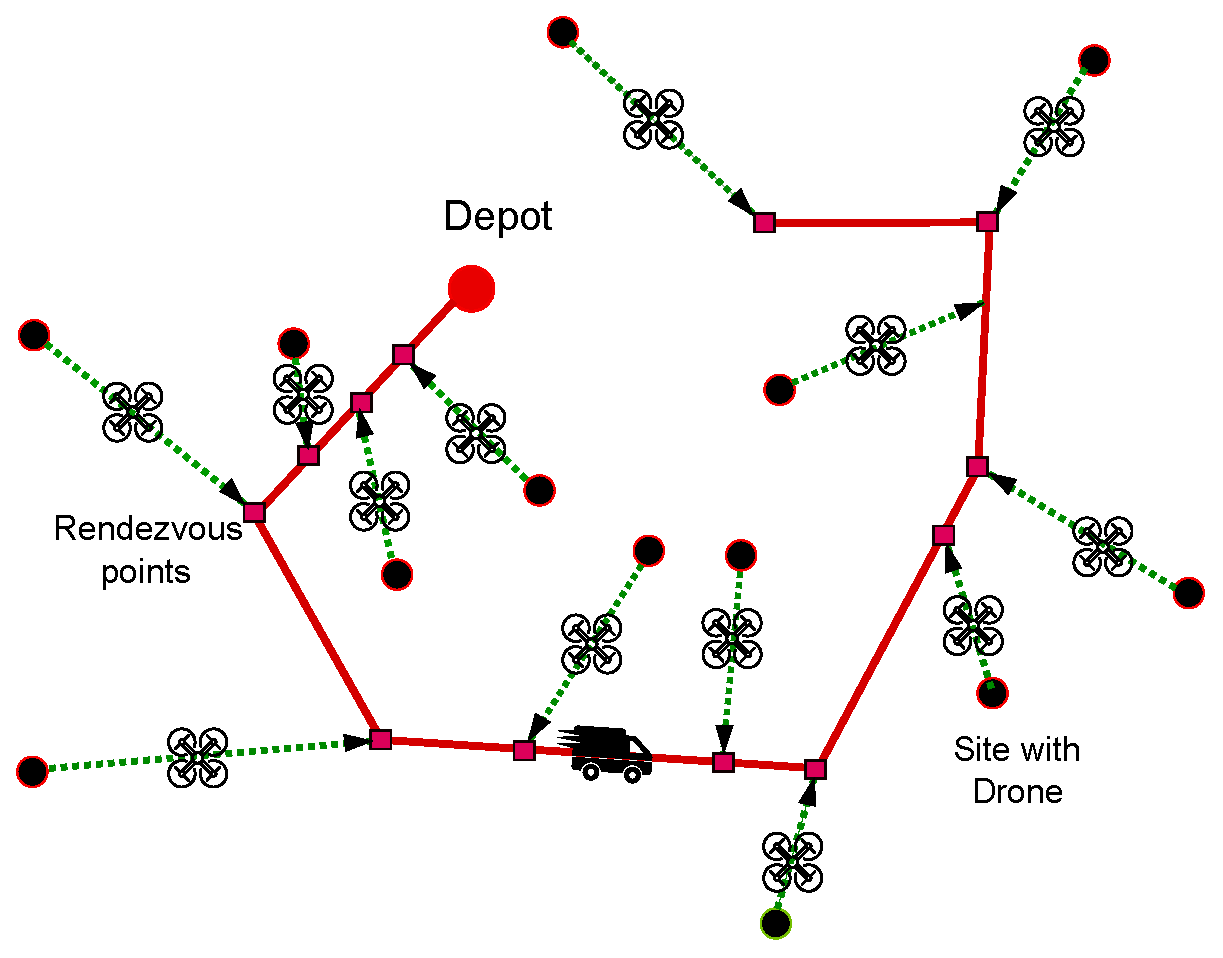
\includegraphics[width=10.0cm]{slide_imgs/reverse_horsefly.eps}
  \end{figure}

\end{frame}

%%%%%%%%%%%%%%%%%%%%%%%%%%%%%%%%%%%%%%%%%%%%%%%%%%%%%%%%%%%%%%%%%%%%%%%%%%

\begin{frame}{Variants: Fixed Truck Route}
\begin{figure}
    \centering
        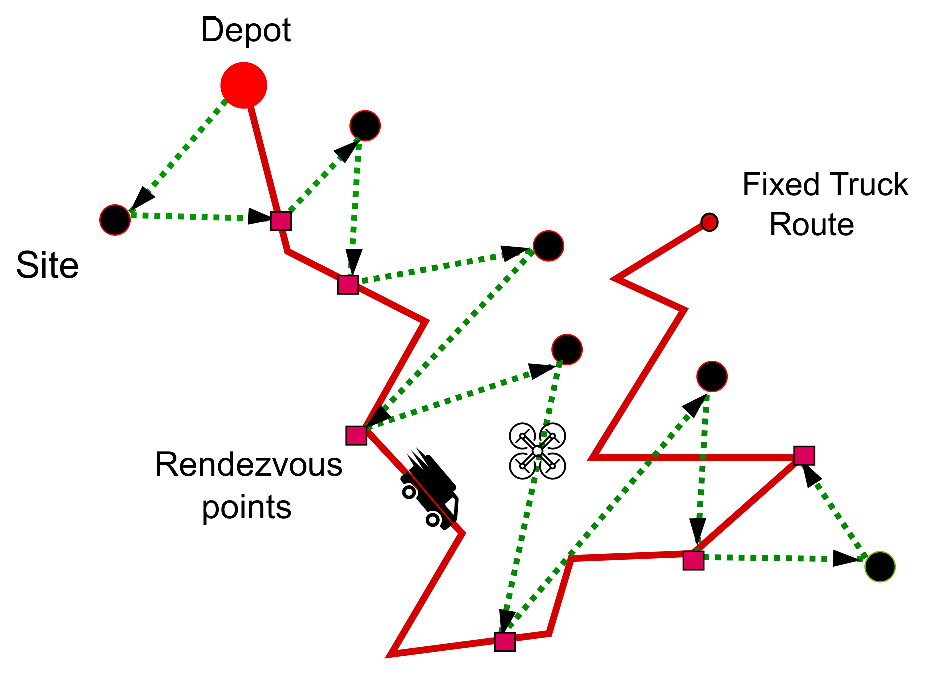
\includegraphics[width=8.0cm]{slide_imgs/fixed_truck_route_variant.eps}
  \end{figure}

\end{frame}

%%%%%%%%%%%%%%%%%%%%%%%%%%%%%%%%%%%%%%%%%%%%%%%%%%%%%%%%%%%%%%%%%%%%%%%%%%%

\begin{frame}{Variants: Segment Horsefly}
\begin{figure}
    \centering
        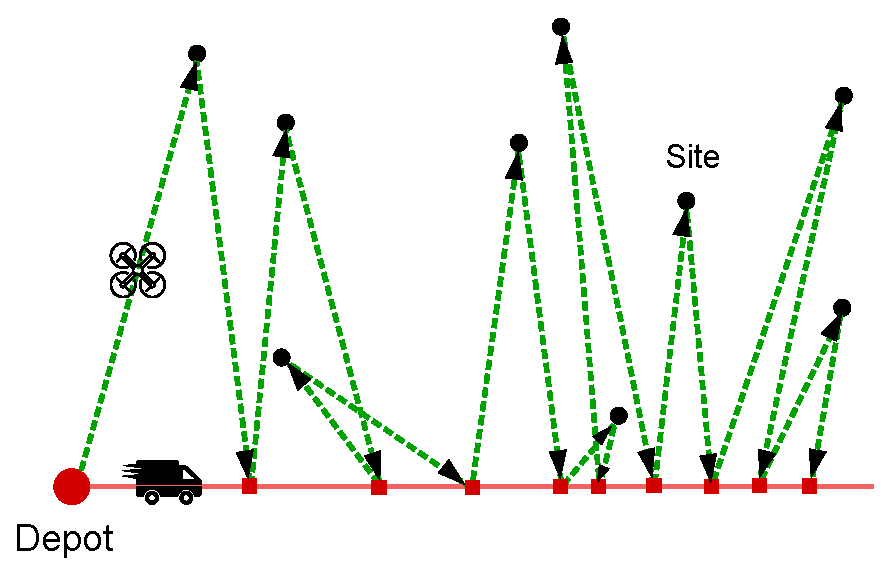
\includegraphics[width=8.0cm]{slide_imgs/segment_horsefly.eps}
  \end{figure}

\end{frame}

%%%%%%%%%%%%%%%%%%%%%%%%%%%%%%%%%%%%%%%%%%%%%%%%%%%%%%%%%%%%%%%%%%%%%%%%%%%%

\begin{frame}[t]{Variants: Multiple Drones}
  \vspace{-10pt}
\begin{figure}
    \centering
        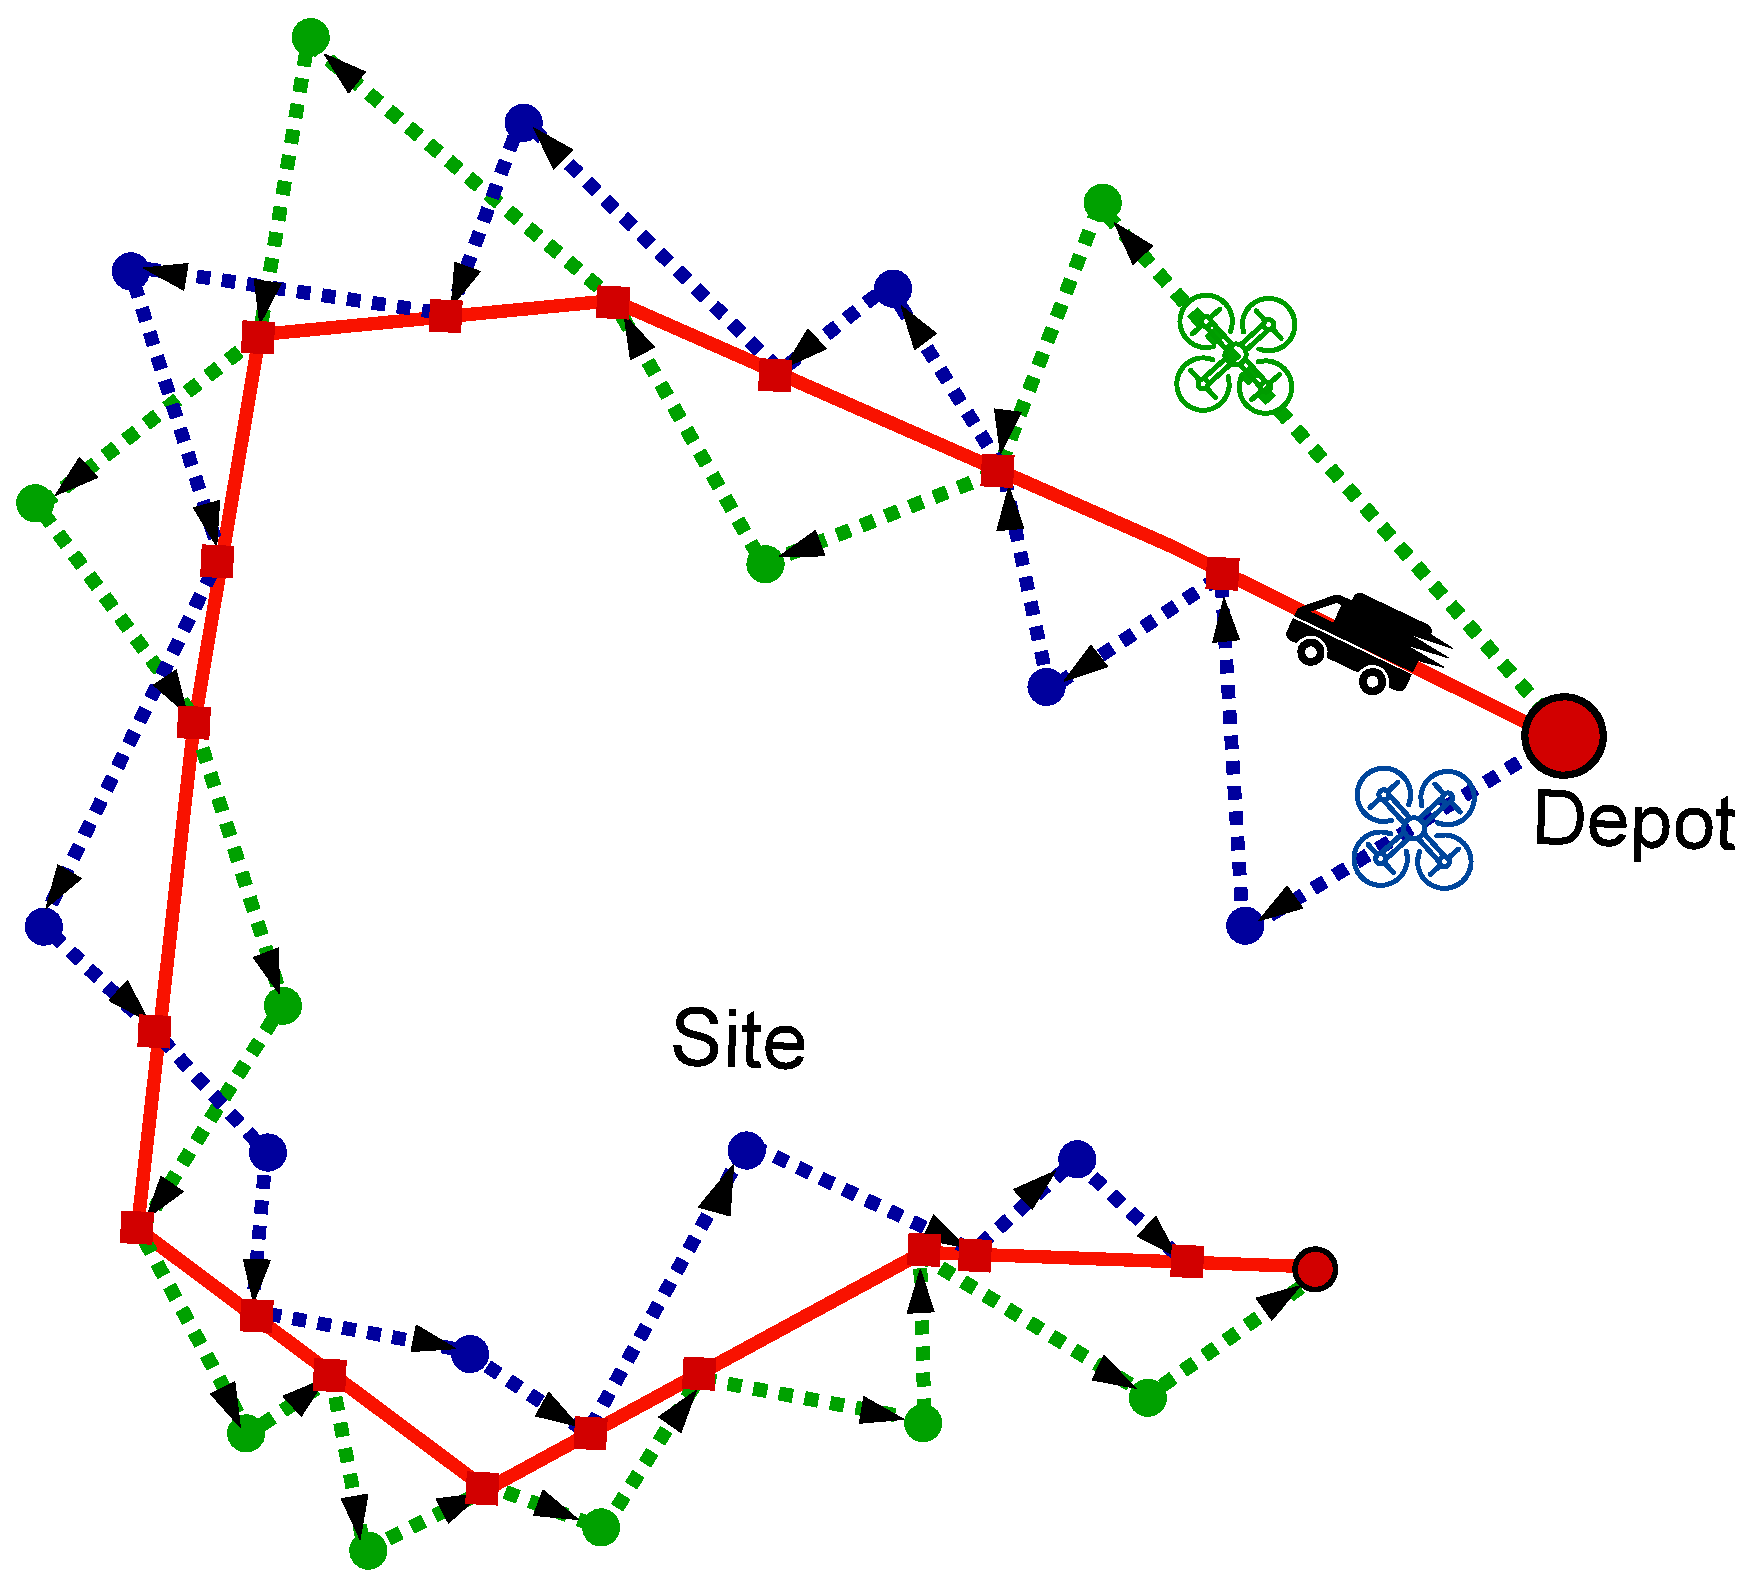
\includegraphics[width=9.0cm]{slide_imgs/multiple_drones.eps}
  \end{figure}
\end{frame}

%%%%%%%%%%%%%%%%%%%%%%%%%%%%%%%%%%%%%%%%%%%%%%%%%%%%%%%%%%%%%%%%%%%%%%%%%%%%%%

\begin{frame}{Summary}
  \begin{center}
    \begin{itemize}
      \item An interesting problem introduced involving 2 heterogenous vehicles. (coordinated vehicle routing).
      \item An implementation of some heuristics for the horsefly problem (Greedy, K2means).
      \item An $O( \log n)$ approximation algorithm. 
      \item Experiments comparing various heuristics. 
      \item Several interesting variants. 
   \end{itemize}
  \end{center}
\end{frame}

\end{document}